\documentclass[a4paper,11pt,twoside,openright]{unibo}

\usepackage[italian]{babel}
\usepackage{newlfont}
\usepackage{url}
\usepackage[backref]{hyperref}
\usepackage{amsthm}
\usepackage{amsmath}
\usepackage{acronym}
\usepackage{graphicx}

%\textwidth=450pt
%\oddsidemargin=0pt

\newtheorem{definitions}{Definizione}[chapter]
\newtheorem{theorem}{Teorema}[chapter]

\acrodef{seti}[SETI]{Search for Extraterrestrial Intelligence}
\acrodef{ipp}[IPP]{Integrated Performance Primitives}
\acrodef{FFT}[FFT]{Fast Fourier Transform}
\acrodef{IDE}[IDE]{Integrated Development Environment}
\acrodef{SIMD}[SIMD]{Single Instruction, Multiple Data }
\acrodef{SSE}[SSE]{Streaming SIMD Extensions}

\graphicspath{{./images/}}

% Remove borders from URLs
\hypersetup{pdfborder = {0 0 0 0}}

\newcommand{\CC}{C\nolinebreak\hspace{-.05em}\raisebox{.4ex}{\tiny\bf +}\nolinebreak\hspace{-.10em}\raisebox{.4ex}{\tiny\bf +}}

\begin{document}
\title{Sviluppo di un software per l'analisi real-time di dati
radioastronomici su macchine multicore}
\author{St\'ephane Bisinger}
\date{May 2010}
\acyear{2009 --- 2010}
\supervisor{Antonella Carbonaro}
\thsubject{Programmazione}
\thsession{Prima}
\pagenumbering{roman}

\maketitle
%\include{frontpage}

\tableofcontents
\listoffigures

\chapter*{Introduzione}
\label{intro}
\addcontentsline{toc}{chapter}{Introduzione}

L'analisi dei segnali \`e un aspetto fondamentale per la cultura moderna: grazie
ad essa esistono telefoni, radio, televisioni, Internet e tanto altro. Grazie
all'analisi dei segnali \`e possibile riprodurre, modificare e creare audio,
immagini, video e tanto altro con l'utilizzo di un computer. Inoltre lo studio
dei segnali elettromagnetici permette di capire molto meglio il mondo attorno a
noi ed ha aperto nuove possibilit\`a per lo studio dei corpi celesti: osservare
un oggetto astronomico con il solo ausilio di strumenti ottici, infatti, non
permette di cogliere moltissimi aspetti che possiamo dedurre dallo studio della
radiazione elettromagnetica proveniente dalla sorgente e dalle zone limitrofe.
Inoltre l'analisi dei segnali offre la possibilit\`a di studiare tanti altri
oggetti come buchi neri, stelle di neutroni, pulsar, redshift e tanto altro. Lo
studio di questi grandi oggetti astronomici ci permette anche di capire molto di
pi\`u la natura della materia ed il suo comportamento in situazioni estreme.

L'analisi dei segnali con mezzi informatici \`e precedente all'introduzione di
personal computers: gran parte di questo lavoro viene svolto su circuiti
elettronici costruiti su misura per effettuare le operazioni necessarie, senza
il bisogno di un calcolatore generico e di programmazione software. Questa
soluzione, ancora largamente in uso al giorno d'oggi, permette di ottenere delle
prestazioni altissime, ma ha il grande difetto di essere poco flessibile e molto
costosa: una piccola modifica quasi insignificante all'algoritmo pu\`o
significare ore e ore di lavoro specializzato. Per questo motivo si cercano al
giorno d'oggi delle soluzioni software in grado di ottenere delle prestazioni
sufficientemente buone da poter fare a meno di elaboratori DSP, cos\`i che si
possa sostituire almeno in parte questo hardware specializzato con generici
elaboratori. Il progetto sviluppato nasce proprio nell'ottica di ottenere buone
prestazioni da un normale elaboratore allo scopo di abbattere i costi in alcuni
campi di ricerca.
\section*{Stazione Radioastronomica di Medicina}
\begin{figure}[htb]
	\begin{center}
		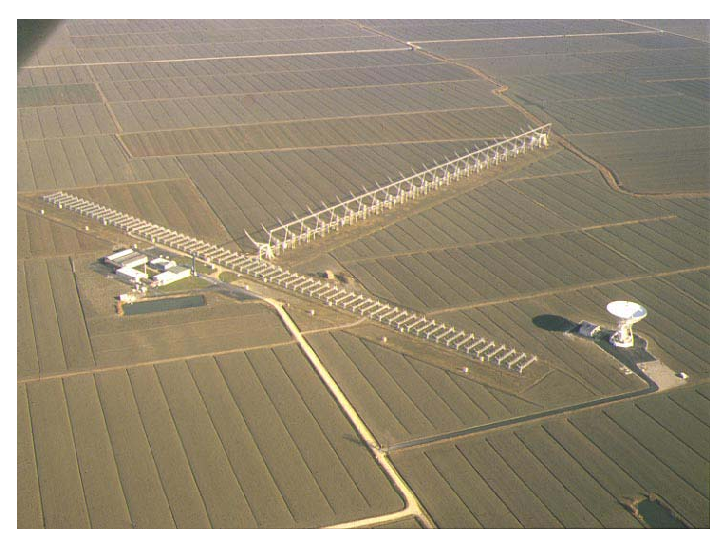
\includegraphics[width=1\linewidth]{antenne}
	\end{center}
	\caption{Veduta aerea della Croce del Nord e dell'antenna parabolica}
	\label{fig:rtscopes}
\end{figure}
Inaugurata nel 1964, la stazione ``Croce del Nord'' di Medicina (BO) ha sancito
l'inizio dell'osservazione radioastronomica in Italia, essendo il primo
osservatorio astronomico fornita di radiotelescopio invece di telescopi ottici.
Un radiotelescopio, a differenza di un telescopio ottico, non osserva i corpi
celesti tramite la parte visibile dello spettro elettromagnetico, ma li osserva
attraverso la captazione di onde radio e la loro trasformazione in segnali
elettrici. Questi segnali elettrici vengono poi elaborati per permettere
l'analisi dello spettro elettromagnetico degli oggetti osservati. I
radiotelescopi presenti a Medicina sono due: una \`e la ``Croce del Nord'', che
d\`a il nome alla stazione, formata da due serie di antenne; l'altra \`e
l'antenna parabolica, dal diametro di 32 metri.

La ``Croce del Nord'' \`e un array di antenne ad apertura, con specchio di forma
cilidrico-parabolica, composto da un braccio orientato in direzione Est--Ovest
ed un braccio orientato in direzione Nord--Sud. Il braccio E/W \`e costituito da
24 cilindri dal diametro di 29 metri e lunghi 24 metri ciascuno, mentre il ramo
N/S \`e costituito da 64 cilindri  di 7,5 metri di diametro e 22 metri di
lunghezza, per un totale di 30000 $m^2$ di area collectrice, che rende la
``Croce del Nord'' uno dei pi\`u grandi radiotelescopi attualmente esistenti sul
pianeta. La ``Croce del Nord'' lavora su segnali centrati a 408 Mhz, con
larghezza di banda che varia dai 2,5 ai 16 Mhz. La sua sensibilit\`a a segnali
anche piuttosto deboli la rende molto utile nello studio di corpi molto
distanti, al di fuori della nostra galassia. Potendo ruotare in una unica
direzione, questo radioscopio pu\`o osservare solamente segnali che transitano
sulla verticale del meridiano in cui si trova, cio\`e \`e un radiotelescopio di
\emph{transito}.

L'antenna parabolica, invece, pu\`o essere orientata in tutte le
direzioni e per questo motivo \`e possibile osservare tutti gli oggetti celesti
presenti nel cielo visibile. Questa antenna, con un diametro di 32 metri, lavora
con frequenze comprese tra i 327 Mhz ed i 43 Ghz. Ha due principali modalit\`a
operative: in rete o in \emph{single dish}.

La parabola partecipa al progetto \ac{VLBI} che, tramite la rilevazione
simultanea di diverse antenne paraboliche situate in posti diversi, permette di
raggiungere una precisione maggiore: correlando i risultati dei diversi
radiotelescopi si riesce ad ottenere una risoluzione equivalente ad una antenna
di dimensione pari alla distanza delle antenne coinvolte. Le osservazioni
particolarmente interessanti da effettuare in questa maniera sono due: la prima
prevede l'osservazione di un stesso oggetto noto da parte di radiotelescopi
situati su placche tettoniche diverse, in modo da studiare il fenomeno della
deriva dei continenti: questo tipo di osservazioni non rientrano
nell'astronomia, ma nella geodinamica, anche se sfrutta un radiotelescopio per
fare i suoi rilevamenti. Il secondo tipo di osservazioni prevede l'osservazione
della posizione e delle propriet\`a chimico-fisiche di un corpo celeste. Durante
circa 4 mesi all'anno l'antenna parabolica di Medicina \`e riservata al progetto
\ac{VLBI}.

Nella modalit\`a \emph{single dish} l'antenna parabolica viene utilizzata in
modo indipendente rispetto ad altre antenne, senza correlare i dati rilevati con
altri dati. In questa modalit\`a si effettuano ad esempio ricerche di comete e
il progetto \ac{seti}.

\section*{Il progetto \ac{seti}}
Nel 1959 due fisici, Giuseppe Cocconi e Philip Morrison, pubblicarono su
\emph{Nature} un articolo in cui ponevano le basi teoriche con cui condurre
ricerche su forme di vita intelligenti extra-terrestri. Secondo questi due
scienziati, se una civilt\`a extra-terrestre evoluta volesse mettersi in
contatto con altri mondi, invierebbe segnali a banda stretta alla frequenza di
1420 Mhz: questa frequenza corrisponde all'emissione spontanea di radiazione
degli atomi di idrogeno neutro, l'elemento pi\`u diffuso nell'universo e il
pi\`u importante sotto molti aspetti di ricerca astronomica. Questa frequenza ha
anche il vantaggio di essere poco soggetta al rumore di fondo presente
nell'universo, quindi di riuscire a viaggiare a grande distanza. Inoltre un
segnale a banda stretta \`e riconosibile molto facilmente rispetto ai segnali a
banda larga emessi naturalmente dai corpi celesti, quindi la ricezione di un
segnale a banda stretta ha buone probabilit\`a di indicare una qualche emissione
artificiale.

In seguito all'articolo di Cocconi e Morrison, nel 1960 Frank Drake punt\`o un
radiotelescopio sulle stelle Tau Ceti ed Epsilon Erinadi: queste due stelle sono
di dimensioni simili al sole ed hanno probabilmente un sistema planetario simile
al sistema solare, quindi hanno una certa possibilit\`a di aver sviluppato la
vita. Bench\'e la sua ricerca non produsse esiti positivi, essa gener\`o
entusiasmo nella comunit\`a astronomica e diversi progetti simili furono avviati
da appassionati durante i tempi liberi dei propri radiotelescopi.
Nel 1961 Drake propose un'equazione per valutare quante forme di vita potrebbero
essere presenti nell'universo:
\[
N = R_* \cdot f_p \cdot n_e \cdot f_l \cdot f_i \cdot f_t \cdot L
\]
Dove:
\begin{itemize}
    \item $R_*$ \`e il numero di stelle di tipo solare che nascono nell'universo
    ogni anno.
    \item $f_p$ \`e la frazione di queste stelle che possiedono un sistema
    planerario.
    \item $n_e$ \`e il numero di pianeti per ogni sistema che si trovano ad una
    distanza adeguata per renderli abitabili.
    \item $f_l$ \`e la frazione di questi pianeti che hanno forme di vita,
    seppur primitive.
    \item $f_i$ \`e la frazione di pianeti con forme di vita intelligente.
    \item $f_t$ \`e la frazione di pianeti su cui l'avanzamento tecnologico
    permette la comunicazione con altri pianeti.
    \item $L$ indica la durata media in anni di tali civilt\`a.
\end{itemize}

Nonostante le stime di Drake indichino numerose civilt\`a presenti
nell'universo, questa equazione mostra anche i grandi problemi legati alla
ricerca \ac{seti}: molte di queste variabili sono quasi impossibili da stimare
basandosi sulla nostra conoscenza attuale dell'universo e molti altri fattori
(come ad esempio la distanza dalla Terra) non sono inclusi. Nonostante questo il
progetto prende piede e negli anni '70 anche la NASA inizia ad interessarsene,
finch\'e nel 1992 non lancia il proprio progetto \ac{seti}. In seguito la NASA
se ne disinteresser\`a ed il progetto continuer\`a solamente grazie a
finanziamenti privati ed il lavoro di volontari all'interno di osservatori
radioastronomici.

\subsection*{\ac{ITASEL}}
In Italia, ed in particolare a Medicina, la ricerca di forme di vita
extraterrestri avviene attraverso il progetto \ac{ITASEL}.

\subsection*{\ac{SERENDIP}}
Analizzare i segnali per il progetto \ac{seti} richiede un sistema informatico
in grado di effettuare i calcoli e le trasformazioni necessarie. L'Universit\`a
di Berkeley, California, ha sviluppato il sistema \ac{SERENDIP}, attualmente
alla versione IV, che permette di analizzare i segnali in modalit\`a \emph{piggy
back}, cio\`e contemporaneamente ad altre elaborazioni senza modificare il
segnale originario. In questo modo non \`e necessario dedicare del tempo di
antenna al progetto \ac{seti}, ma \`e possibile fare le osservazioni durante
altri progetti di ricerca senza interferenze: questo ha permesso di abbattere
notevolmente i costi del progetto, oltre a sfruttare tutto il tempo di utilizzo
dell'antenna. Con questo spettrometro \`e possibile analizzare segnali a 24
milioni di canali con larghezza di banda di 15 Mhz.

\section*{Il progetto}
Il progetto consiste nello sviluppo di uno spettrometro, scritto nel linguaggio
di programmazione \CC, allo scopo di ottenere le migliori prestazioni possibili
sfruttando unicamente un elaboratore generico in contrapposizione ad un
processore DSP. Questo spettrometro pu\`o trovare applicazione in diversi ambiti
di ricerca, incluso il progetto \ac{seti}, dove pu\`o essere paragonato alle
prestazioni di \ac{SERENDIP} IV.

Un requisito fondamentale di questo progetto \`e che sia sufficientemente
modulare da permettere una sua estensione e per permettere l'introduzione di
filtri e altre trasformazioni sui segnali senza dover riscrivere codice gi\`a
esistente, ma sfruttando delle interfacce predefinite.

Per raggiungere questi scopi \`e stato dedicato ampio tempo alla progettazione
del software, in modo che si potesse procedere allo sviluppo con le idee chiare
sulla struttura da adottare nel progetto.

Nei capitoli seguenti verranno illustrati alcuni concetti matematici di base
fondamentali per la comprensione del lavoro svolto, per poi procedere
all'analisi della fase di progettazione e quella di sviluppo. Verranno poi
mostrati i risultati raggiunti e tratte le relative conclusioni anche in
relazione agli obiettivi posti. Saranno poi indicati alcuni dei possibili
sviluppi futuri, ottimi punti di partenza per altri lavori di tesi o di
tirocinio per altri studenti.

\chapter{Basi di elaborazione del segnale}
\pagenumbering{arabic}
\label{math_bkg}
In questo capitolo introdurremo alcuni concetti basilari sull'elaborazione dei
segnali necessari alla comprensione del funzionamento di uno
spettrometro e del suo campo di applicazione. Sapere cosa sia un segnale, come
si estraggono ed elaborano le informazioni in esso contenuto, quali siano i
concetti matematici utilizzati \`e fondamentale per capire il lavoro svolto.\\
Questo materiale introduttivo \`e sufficiente per avere una panoramica sui
concetti teorici utilizzati.

\section{Segnali}
Il nostro corpo \`e in grado di percepire, attraverso i sensi, alcune delle
variazioni nelle propriet\`a fisiche del mondo che ci circonda. Queste variazioni che percepiamo vengono
elaborate dal nostro cervello che riesce a ricavarne informazioni utili: In questo modo
siamo in grado di percepire se fa caldo o freddo, se c'\`e luce, se un oggetto
\`e di un colore piuttosto che un altro, ecc. Va notato che in questi segnali
c'\`e una componente fisica (la temperatura) e l'informazione veicolata
(freddo/caldo). \cite{bertoni}
\begin{definitions} \label{def:signal}
Si dice segnale una qualunque quantit\`a che varia nel tempo o nello spazio.
\end{definitions}
Secondo la precedente definizione, quindi, \`e possibile che un segnale non
contenga informazioni utili: in questo caso ci si riferisce al segnale come
\emph{rumore}. Il rumore \`e anche una componente di interferenza o errore su di
un segnale che si cerca di interpretare.

Un segnale viene quindi rappresentato da una funzione $g = f(c)$, ove:
\begin{itemize}
    \item $g$ \`e una variabile dipendente su di una grandezza fisica in
    relazione al tempo o spazio.
    \item $c$ \`e una varaibile indipendente che rappresenta lo spazio o il
    tempo.
    \item $f$ \`e una funzione che associa ad un valore temporale o spaziale $c$
    la corrispondente quantit\`a $g$.
\end{itemize}

Per semplicit\`a di esposizione, d'ora in avanti si far\`a riferimento
unicamente a segnali in relazione al tempo.

\subsection{Segnali periodici}
Una importante classe di segnali sono i segnali periodici. Un segnale \`e
periodico se si ripete in un certo periodo di tempo: definendo $T$ il periodo con
cui si ripete il segnale e con $t$ un qualunque momento nel tempo, per ogni $k$,
vale $f(t) = f(t + kT)$. Un segnale periodico $f(t)$ \`e quindi univocamente
individuato nell'intervallo $\frac{T}{2} \le t \le \frac{T}{2}$.

Si definisce  \emph{frequenza} di un segnale periodico $f(t)$ il numero di
ripetizioni del periodo $T$ nell'unit\`a di tempo. Risulta quindi:
\[
\nu = \frac{1}{T}
\]
L'unit\`a di misura della frequenza \`e l'Hertz ed indica il numero di cicli
(ripetizioni) al secondo.

\subsection{Frequenza radio}
I segnali elettromagnetici vengono classificati a seconda della loro frequenza
in diverse categorie:
\begin{itemize} 
	\item Frequenze minori di 3 GHz vengono denominate \emph{frequenze radio}.
	\item Frequenze comprese tra 3 GHz e 300 GHz sono denominate
		\emph{microonde}.
	\item Frequenze comprese tra 300 GHz e 400 000 GHz (400 THz) sono denominate
		\emph{infrarossi}.
	\item Frequenze comprese tra 400 THz e 750 THz sono parte dello
		\emph{spettro visibile}.
	\item Frequenze comprese tra 750 THz e 30 000 THz (30 PHz) sono denominate
		\emph{raggi ultravioletti}.
	\item Frequenze comprese tra 30 Phz e 30 000 PHz (30 EHz) sono denominate
		\emph{Raggi X}.
	\item Frequenze superiori ai 30 EHz sono denominate \emph{Raggi Gamma}.
\end{itemize}
Va notato che questi limiti sono solo convenzionali e non hanno una definizione
standard.

\subsubsection{Studio dei corpi celesti}
\begin{figure}[htb]
	\begin{center}
		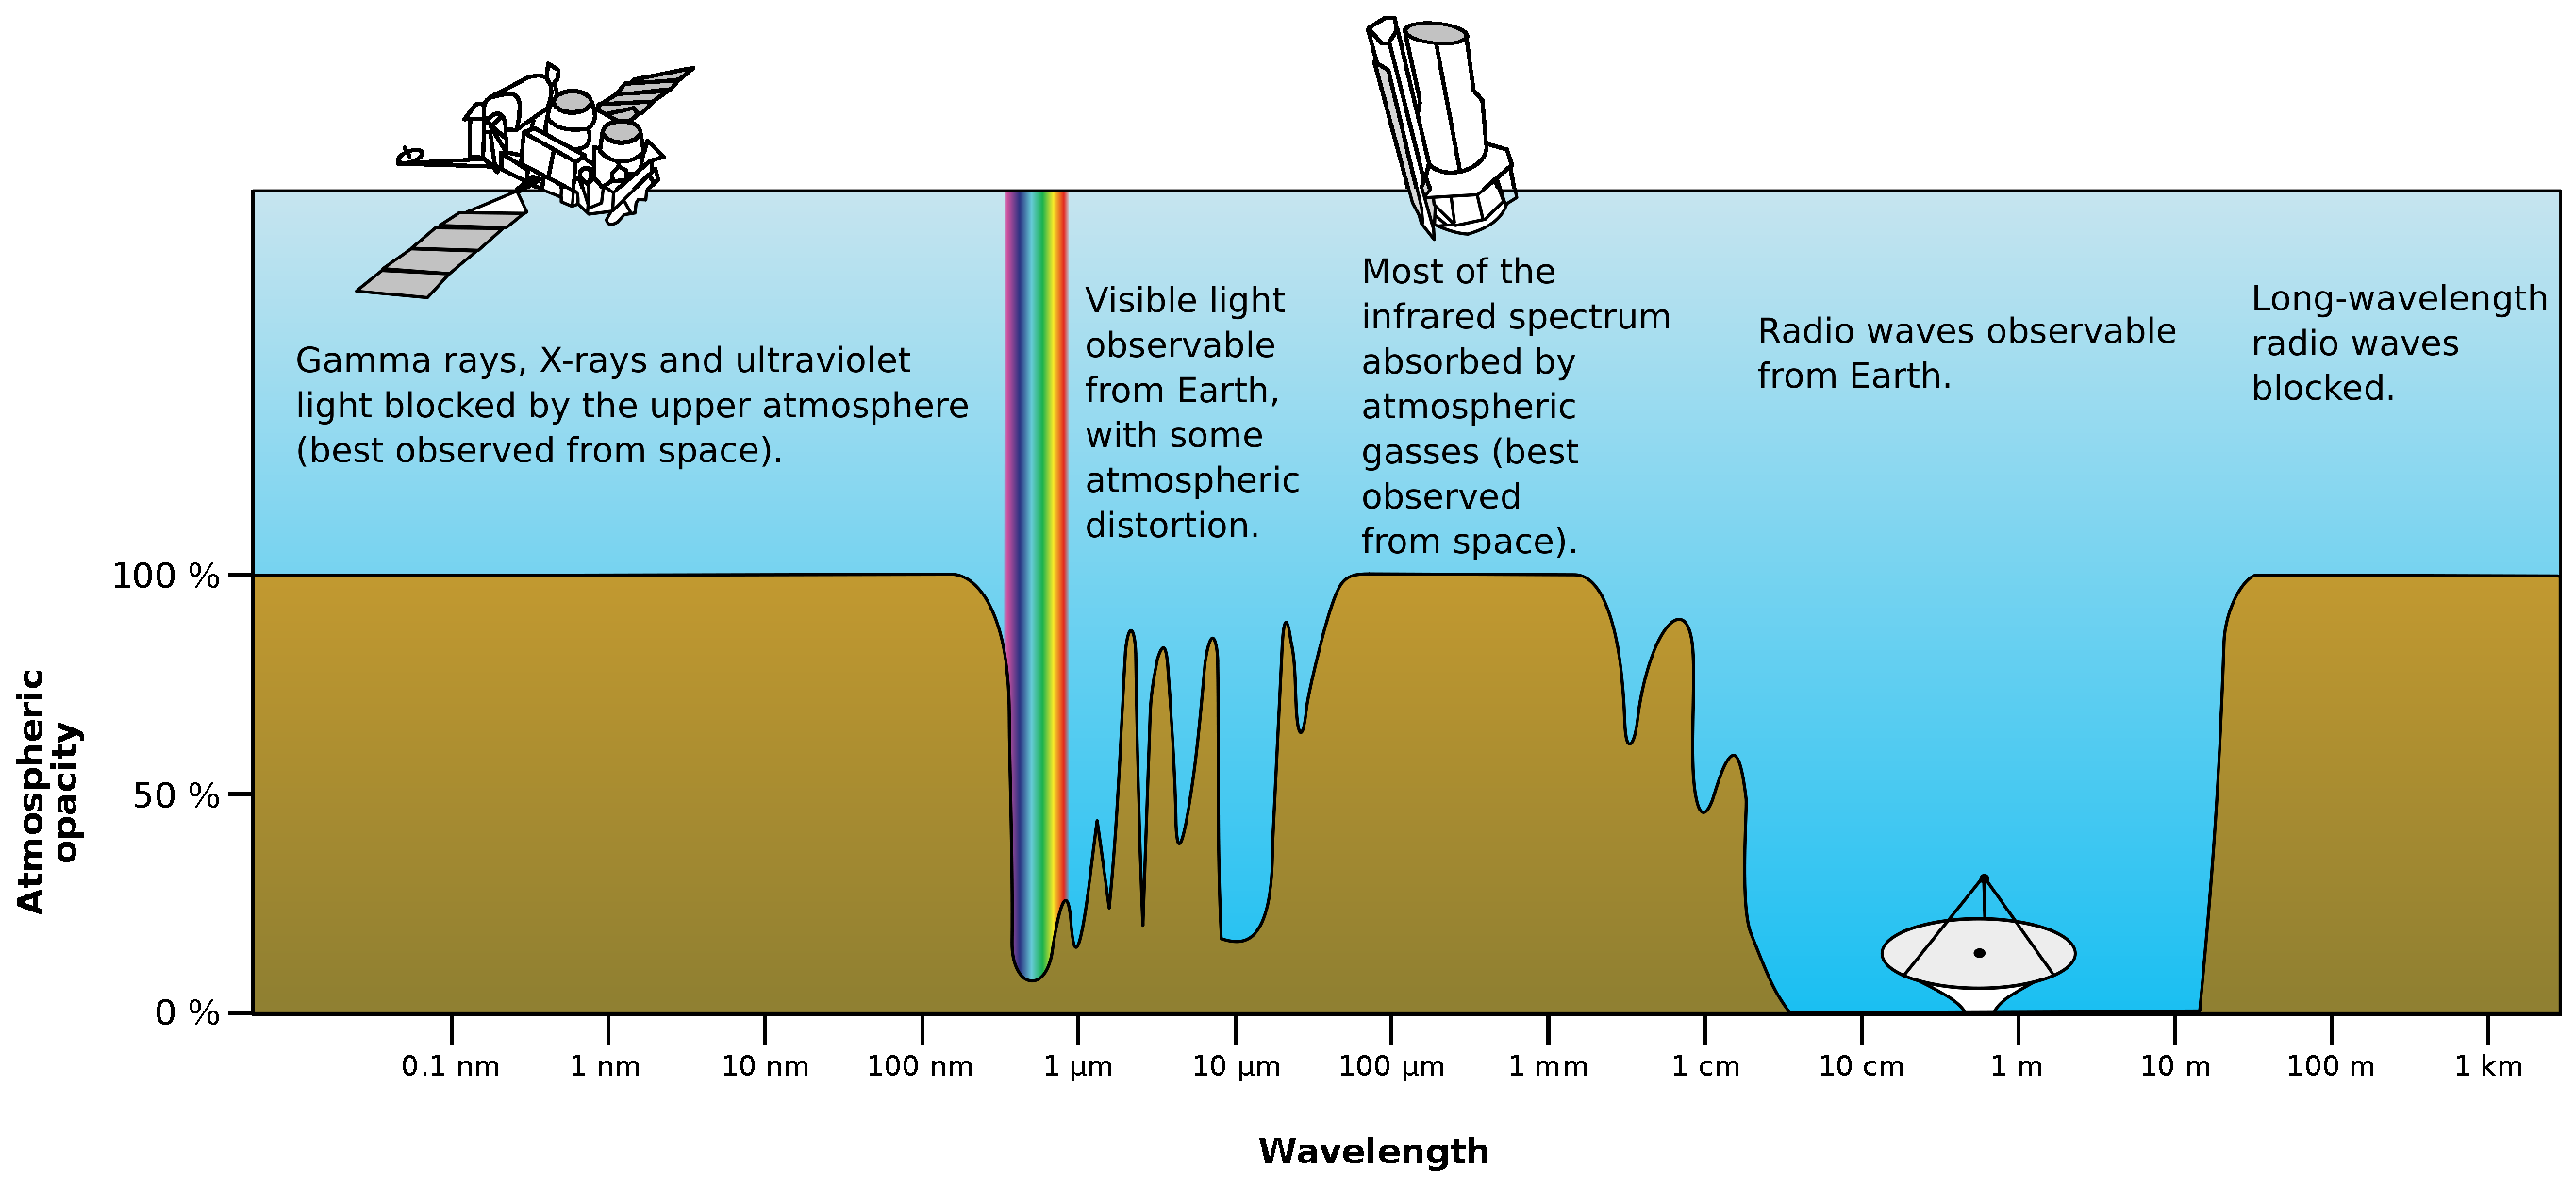
\includegraphics[width=1\linewidth]{Atmospheric_electromagnetic_opacity}
	\end{center}
	\caption{Permeazione dei segnali elettromagnetici nell'atmosfera}
	\label{fig:atm_em_op}
\end{figure}
I segnali elettromagnetici sono fondamentali per lo studio dei corpi celesti.
Tuttavia va considerata la permeabilit\`a dell'atmosfera terrestre rispetto ai
segnali che ci arrivano dallo spazio, come illustrato in Figura
\ref{fig:atm_em_op}\footnote{Fonte:
\url{http://coolcosmos.ipac.caltech.edu/cosmic_classroom/cosmic_reference/irwindows.html}}:
come si pu\`o notare, lo studio dei corpi celesti da terra \`e possibile solo
nello spettro visibile (telescopi, con qualche distorsione) oppure nello spettro
delle frequenze radio (radiotelescopi). Per altre lunghezze d'onda, \`e
necessario studiare questi segnali direttamente dallo spazio con l'ausilio di
satelliti. I moderni radiotelescopi lavorano tra i 70 Mhz ed i 43 Ghz, a seconda
del radiotelescopio, quindi anche le microonde rivestono una qualche importanza
nello studio dei corpi celesti. Questi tipi di segnale sono oggetto di
elaborazione del software sviluppato.

\section{ADC: Analog--to--Digital Conversion}
Per interpretare i segnali del mondo che ci circonda, possiamo sfruttare la
velocit\`a di calcolo di un elboratore; tuttavia per poterlo usare, bisogna
essere in grado di rappresentare le informazioni che riceviamo in modo che
l'elaboratore sia in grado di capirle. Per questo motivo dobbiamo trovare un
modo di trasformare un segnale \emph{analogico} in un segnale \emph{digitale}.

\subsection{Segnali analogici, segnali digitali}
Come abbiamo visto nella definzione \ref{def:signal}, i segnali hanno due
componenti: il tempo e il valore assunto dalla grandezza fisica che osserviamo.
Queste due componenti possono assumere un qualunque valore reale, cio\`e il
segnale ha \emph{tempo continuo} e \emph{valori continui}. Tuttavia, in questo
modo il segnale non pu\`o essere rappresentato da un elaboratore, in quanto un
elaboratore pu\`o contenere solamente quantit\`a finite, mentre le componenti
del segnale sono quantit\`a infinite. Per questo motivo bisogna cercare di far
rientrare il segnale in un range di valori finiti e renderlo cos\`i
rappresentabile da un calcolatore.

Per rendere finita la misurazione del tempo, si possono salvare i valori
rilevati ad un intervallo prefissato, ad esempio una volta ogni secondo.
Misurando un segnale per 10 secondi si otterranno cos\`i 10 valori associati ad
ogni secondo. Un segnale di questo tipo ha \emph{tempo discreto}, ma valori
ancora \emph{continui}. Un dispositivo che raccoglie valori con una determinata
frequenza si chiama \emph{campionatore}.

Per rendere i valori finiti, si pu\`o scegliere di utilizzare un certo insieme
di grandezze, ad esempio $1$ e $-1$, e per ogni valore rilevato, associare la
grandezza pi\`u vicina. Quindi se rileviamo i valori $4$, $10$, $-5$ e $-13$,
salviamo il segnale con i valori $1$, $1$, $-1$, $-1$. Cos\`i facendo, il
segnale assume \emph{valori finiti} che sono rappresentabili in un elaboratore,
nell'esempio fatto con l'uso di 1 bit. Un dispositivo che associa ai valori
rilevati il pi\`u vicino valore rappresentabile dall'elaboratore si chiama
\emph{quantizzatore}.

Un segnale che ha tempo \emph{continuo} e valori \emph{continui} si chiama
\emph{segnale analogico}, mentre un segnale con tempo \emph{discreto} e valori
\emph{finiti} si chiama \emph{segnale digitale}.

Come \`e facile intuire, la conversione da analogico a digitale pu\`o introdurre
degli \emph{errori}, cio\`e del \emph{rumore}, in quanto la versione digitale di
un segnale analogico \`e una approssimazione. Fortunatamente \`e possibile
valutare questo margine di errore e ridurlo a seconda delle necessit\`a sia
aumentando il numero di bit usati per rappresentare i valori nel tempo, sia
aumentando il numero di rilevazioni effettuate nello spazio temporale di
osservazione.

\subsection{Teorema del Campionamento}
Quando si effettua il campionamento di un segnale $f(t)$, si sceglie un periodo
$\tau$ e si fanno $n$ misurazioni nel tempo, ottenendo quindi un segnale di
tipo $f(n\tau)$. Come possiamo assicurarci che da $f(n\tau)$ sia possibile
ricostruire il segnale originale $f(t)$?
Il teorema del campionamento fornisce una risposta definendo un limite basato
sulla frequenza massima del segnale:
\begin{theorem} \label{the:nyquist}
	Un segnale $f(t)$ con frequenza massima $\nu_m$ pu\`o essere ricostruito dal
	segnale campionato $s(n\tau)$ con frequenza $\nu_s = \frac{1}{\tau}$ se
	$\nu_s > 2\nu_m$
\end{theorem}
Cio\`e la frequenza di campionamento deve essere doppia rispetto alla frequenza
massima presente nel segnale.\footnote{Per una dimostrazione del teorema del
campionamento, fare riferimento a \cite{MDFT07}} Nel caso in cui un segnale venga campionato con
frequenza di campionamento $\nu_s < 2\nu_m$, si verifica un fenomeno di
\emph{aliasing}, cio\`e le componenti a frequenza maggiore di $\frac{\nu_s}{2}$
verranno ricostruite come se avessero un'altra frequenza compresa tra $0$ e
$\frac{\nu_s}{2}$; a questo modo l'intero segnale verrebbe compromesso e sarebbe
impossibile recuperare il segnale originario. Per evitare che ci\`o accada si
applica un filtro al segnale che deve essere campionato per eliminare tutte le
frequenze maggiori di $\frac{\nu_s}{2}$, evitando che frequenze non di nostro
interesse possano interferire con le frequenze che andremo ad elaborare.

\section{La Trasformata Discreta di Fourier}
\subsection{Introduzione alla Trasformata di Fourier}
Jean Baptiste Joseph Fourier, vissuto a cavallo tra il XVIII e IX secolo, era
un matematico francese che, presentando i suoi  studi sulla propagazione del
calore, affermava che qualunque segnale periodico continuo potesse essere
rappresentato come somme pesate di sinusoidi. Questa teoria fu molto osteggiata
da Joseph Louis Lagrange, il quale sosteneva che per segnali contenenti angoli,
come ad esempio le onde quadre, ci\`o non fosse possibile e per questo il
lavoro di Fourier non fu pubblicato per 15 anni, fino alla morte dello stesso
Lagrange.\footnote{cfr. \cite{TSEGDSP97}, capitolo 8} In realt\`a l'approccio di
Fourier non era sbagliato, ma anche l'obiezione di Lagrange \`e valida: se da un
lato \`e vero che un segnale con angoli non potesse essere rappresentato come
somme di sinusoidi, si riesce ad ottenere una approsimazione cos\`i accurata del
segnale da avere una differenza energetica pari a zero.  Questo fenomeno \`e
conosciuto come \emph{Fenomeno di Gibbs}\footnote{cfr.  \cite{TSEGDSP97},
capitolo 11}

\subsection{Tipi di Trasformate di Fourier}
Esistono quattro tipi di segnali possibili, ognuno con la sua trasformata di
Fourier. Un segnale pu\`o essere periodico o aperiodico, continuo o discreto. Ne
conseguono i quattro tipi di trasformate:
\begin{itemize}
	\item \textbf{Aperiodico - Continuo}: Il segnale non ha \`e periodico ed
		assume infiniti valori. Per analizzarlo si utilizza la \emph{Trasformata
		di Fourier}.
	\item \textbf{Periodico - Continuo}: Il segnale assume infiniti valori che
		si ripetono con un certo periodo. In questo caso si usa la \emph{Serie
		di Fourier}.
	\item \textbf{Aperiodico - Discreto}: Il segnale non ha periodo e assume
		solo un numero finito di valori. In questo caso si utilizza la
		\emph{Trasformata di Fourier a tempo discreto}.
	\item \textbf{Periodico - Discreto}: Il segnale assume un numero finito di
		valori che si ripetono con un dato periodo. La trasformata utilizzata
		\`e la \emph{Trasformata discreta di Fourier}.
\end{itemize}
Ogni segnale usato per queste trasformate deve essere infinito; nel caso in cui
ci fosse un segnale discreto con un numero di punti finito, come succede quando
abbiamo un segnale rappresentato all'interno di un elaboratore, si pu\`o
immaginare questo segnale come se fosse infinito. Se si immagina che prima e
dopo del segnale in nostro possesso il segnale abbia un valore pari a 0, si
user\`a la trasformata di Fourier a tempo discreto, altrimenti se si immagina il
segnale infinito come una ripetizione dei dati in nostro possesso, si utlizza la
trasformata discreta di Fourier. Purtroppo, un qualunque segnale aperiodico ha
infinite componenti sinusoidali, quindi la trasformata di Fourier a tempo
discreto non \`e utilizzabile con un elaboratore, lasciando unicamente la
trasformata discreta di Fourier a nostra disposizione.

Ognuna delle quattro trasformate pu\`o essere eseguita nella sua forma
complessa, dove un insieme di numeri complessi vengono trasformati in un'altro
insieme di numeri complessi, oppure nella forma reale, dove un insieme di numeri
reali vengono trasformati in due insiemi di numeri reali. La forma complessa
di una trasformata \`e molto pi\`u difficile da comprendere, perci\`o verr\`a
esposta unicamente la forma reale della trasformata. Analizzeremo unicamente la
versione discreta della trasformata di Fourier in quanto \`e di pi\`u
semplice comprensione, pur essendo concettualmente identica agli altri tipi di
trasformata, oltre ad essere la trasformata utilizzata direttamente nel
progetto.

\subsection{Analisi e Sintesi}
\label{analisi_sintesi}
Quando applichiamo la trasformata di Fourier, non facciamo altro che passare tra
due rappresentazioni diverse dello stesso segnale: il segnale originario \`e nel
dominio del tempo, mentre il segnale trasformato \`e nel dominio delle
frequenze. Esiste anche la trasformata inversa, che permette di passare dal
dominio della frequenza al dominio del tempo.
L'operazione che trasforma un segnale nel dominio del tempo ad uno nel dominio
delle frequenze si chiama \emph{analisi}, \emph{decomposizione} o semplicemente
{trasformata DFT}, mentre l'operazione inversa si chiama \emph{sintesi} o
{trasformata inversa}. Entrambe le operazioni possono essere espresse come
algoritmi ed utilizzate da elaboratori.

Quando rappresentiamo un segnale in un elaboratore, avremo un vettore,
\texttt{x[]}, contente le ampiezze del segnale nei vari intervalli di tempo. Se
al momento del campionamento abbiamo scelto di misurare $N$ campioni, avremo ora
un vettore di $N$ elementi che vanno da 0 a $N$. Di solito per facilitare la
computazione tramite elaboratore $N$ viene scelto tra le potenze di
2\footnote{La \ac{FFT} richiede segnali che abbiano lunghezza pari ad una potenza di
due, per poter funzionare.}. La controparte di questo segnale \`e suddivisa in
due parti, \texttt{ReX[]} contenente i valori per le ampiezze dei coseni
presenti nel segnale, e \texttt{ImX[]} contenente i valori per le ampiezze dei
seni presenti nel segnale.\footnote{Le notazioni \texttt{ReX[]} e \texttt{ImX[]}
significano, rispettivamente, ``parte reale di X'' e ``parte immaginaria di X''.
Questi nomi provengono dalla versione complessa della trasformata, ma in questo
caso i due vettori vanno considerati semplicemente come ampiezze dei coseni e
dei seni presenti nel segnale.} I due vettori \texttt{ReX[]} e \texttt{ImX[]}
contengono $N/2 + 1$ valori ciascuno, partendo da 0 e arrivando a $N/2$.

\subsection{Funzioni base della DFT}
Quando effettuiamo la DFT di un segnale, otteniamo due vettori che rappresentano
l'ampiezza delle funzioni di base della DFT. Queste funzioni base sono le
funzioni coseno e seno di diversa frequenza e ampiezza unitaria che fanno parte
del segnale. Quindi avremo che:
\[
\begin{array}{c}
c_k[i] = \cos\left(\frac{2\pi ki}{N}\right)\\[0.5em]
s_k[i] = \sin\left(\frac{2\pi ki}{N}\right)\\[0.5em]
i = 0\dots N-1, \quad k = 0 \dots N/2
\end{array}
\]
Al variare di $k$, varia la frequenza della sinusoide negli $N$ punti: per $k =
0$ avremo $0$ cicli negli $N$ punti, per $k=1$ avremo 1 ciclo, per $k=2$ ci
saranno due cicli e cos\`i via. Ad ogni $c_k$ ed $s_k$, si associano le relative
ampiezze \texttt{ReX[k]} ed \texttt{ImX[k]}.

Tre aspetti importanti vanno notati:
\begin{itemize}
	\item $\boldsymbol{c_0}$ ha valore 1 per tutti i punti $N$:
		$\cos\left(\frac{2\pi 0i}{N}\right) = \cos(0) = 1, \quad \forall i \in
		(0 \dots N-1)$
	\item $\boldsymbol{s_0}$ ha valore 0 in tutti i punti $N$:
		$\sin\left(\frac{2\pi 0i}{N}\right) = \sin(0) = 0, \quad \forall i \in
		(0 \dots N-1)$
	\item $\boldsymbol{s_{N/2}}$ ha valore 0 in tutti i punti $N$:
		$\sin\left(\frac{2\pi N/2i}{N}\right) = \sin(\pi i) = 0, \quad \forall i \in
		(0 \dots N-1)$
\end{itemize}

In particolare si nota che i valori \texttt{ImX[0]} e \texttt{ImX[N/2]} non
influiscono in nessun modo, quindi vengono generalmente impostati a 0. 

\subsection{DFT inversa}
Per ottenere il segnale originario dal segnale nel dominio delle frequenze basta
effettuare la somma dei coseni e dei seni pesati:
\[
x[i] = \sum_{k=0}^{N/2} Re\bar{X}[k] \cos\left(\frac{2\pi ki}{N}\right) +
\sum_{k=0}^{N/2} Im\bar{X}[k] \sin\left(\frac{2\pi ki}{N}\right)
\]
Nell'equazione si usano le versioni normalizzate dei vettori:
\texttt{ReX[]} e \texttt{ImX[]}:
\[
\begin{array}{l}
	Re\bar{X}[k] = \frac{ReX[k]}{N/2}\\[0.5em]
	Im\bar{X}[k] = -\frac{ImX[k]}{N/2}
\end{array}
\]
Ci sono due casi speciali:
\[
\begin{array}{l l}
	Re\bar{X}[0] & = \frac{ReX[0]}{N} \\[0.5em]
	Re\bar{X}[N/2] & = \frac{ReX[N/2]}{N}
\end{array}
\]
Questa normalizzazione viene introdotta perch\'e il dominio delle frequenze \`e
definito come densit\`a spettrale, cio\`e le frequenze sono divise in bande e
ogni valore \texttt{ReX[]} e \texttt{ImX[]} rappresenta la quantit\`a di segnale
(ampiezza) presente per ogni unit\`a dell'ampiezza di banda: ad esempio il
valore \texttt{ReX[1]} rappresenta l'ampiezza del segnale nella banda 1, che
corrisponde all'intervallo $0,5\dots1,5$, \texttt{ReX[2]} rappresenza l'ampiezza
del segnale nella banda 2 ($1,5\dots2,5$) e cos\`i via. Ci sono $N/2+1$ bande,
quindi ogni banda \`e larga $\frac{1}{N/2} = \frac{2}{N}$, tranne la prima e
l'ultima: la banda 0 ($0\dots 0.5$) e la banda $N/2$ ($N/2-0,5\dots N/2$) sono
larghe esattamente la met\`a, $\frac{1}{N}$.

\subsection{Calcolo della DFT}
Il primo metodo per calcolare la DFT ha solo lo scopo di far comprendere il
procedimento, ma non ha nessuna applicazione pratica in quanto troppo complesso
a livello computazionale. Dato un segnale \texttt{x[]} per calcolare la sua
trasformata possiamo creare $N$ equazioni semplicemente prendendo il primo punto
delle sinusoidi di base e sommarli tra loro. Sappiamo che la loro somma,
moltiplicata per i rispettivi pesi, devono essere uguali al primo punto del
segnale originario. Andando a creare delle equazioni simili per gli altri punti,
otterremo le $N$ equazioni di cui abbiamo bisogno e potremo risolverle usando un
qualunque metodo algebrico, ad esempio il metodo di eliminazione di Gauss.
Supponiamo che il nostro segnale abbia 4 punti:
\begin{align*}
Re\bar{X}[0] + Re\bar{X}[1] + Re\bar{X}[2] & = x[0]\\
Re\bar{X}[0] + Re\bar{X}[1]\cos\left( \frac{\pi}{2} \right) +
Re\bar{X}[2]\cos\left( \pi \right) + Im\bar{X}[1]\sin\left( \frac{\pi}{2}
\right) & = x[1]\\
Re\bar{X}[0] + Re\bar{X}[1]\cos\left( \pi \right) + Re\bar{X}[2]\cos\left( 2\pi
\right) + Im\bar{X}[1]\sin\left( \pi \right) & = x[2]\\
Re\bar{X}[0] + Re\bar{X}[1]\cos\left( \frac{3\pi}{2} \right) +
Re\bar{X}[2]\cos\left( 3\pi \right) + Im\bar{X}[1]\sin\left( \frac{3\pi}{2}
\right) & = x[3]\\
\end{align*}
Ci ritroviamo con 4 variabili e 4 equazioni linearmente indipendenti, quindi
siamo in grado di risolvere queste equazioni e trovare i valori delle
variabili. Purtroppo questo metodo di risoluzione non \`e efficiente e non
viene usato per calcolare la trasformata con l'ausilio di un elaboratore.
\subsection{FFT: Fast Fourier Transform}
\label{fft}
Quando si utilizza un elaboratore per fare dei calcoli, \`e importante valutare
l'efficienza dell'algoritmo utilizzo, cio\`e valutare quanto tempo impiega il
nostro algoritmo per eseguire il calcolo e di quanto cresce il tempo di
esecuzione all'aumentare dei dati inseriti in ingresso. Il calcolo della DFT
tramite correlazione\footnote{cfr. \cite{TSEGDSP97}, capitoli 6---8} richiede un
tempo di esecuzione all'incirca di $k_{DFT}N^2$. $k_{DFT}$  \`e una costante di
proporzionalit\`a rispetto all'algoritmo che con un processore a 100Mhz
equivale a 7 microsecondi, con tutte le ottimizzazioni possibili. Considerando un segnale
di $N = 1024$ punti il tempo di esecuzione \`e di circa 7 secondi. Questo tempo
\`e enorme, soprattutto considerando la piccola dimensione del segnale; per
questo motivo \`e fondamentale trovare un algoritmo pi\`u efficiente nel calcolo
della trasformata di Fourier. La \emph{Fast Fourier Transform} \`e un algoritmo
che, utilizzando un approccio completamente diverso al calcolo della
trasformata, riesce ad ottenere un tempo di esecuzione pari a
$k_{FFT}N\log_{2}N$. In questo caso, $k_{FFT}$ equivale a 10 microsecondi su
processore a 100Mhz, quindi un segnale di $N=1024$ punti viene trasformato in 70
millisecondi.\footnote{Per i dati dei test, cfr. \cite{TSEGDSP97}, capitolo 12}
Comparando i due tempi si capisce che la FFT permette di effettuare calcoli
anche su segnali di dimensioni abbastanza grandi, poich\'e la crescita
logaritmica assicura che il tempo di calcolo non aumenti troppo bruscamente
all'aumentare dei punti.

Un altro vantaggio non indifferente della \ac{FFT} \`e la sua scarsa sensibilit\`a
agli errori di arrotondamento: poich\'e l'algoritmo diminuisce drasticamente il
numero di operazioni da effettuare sui numeri, anche gli errori di
arrotondamento rimangono molto contenuti. Questo assicura una buona stabilit\`a
numerica dell'algoritmo anche con grandi moli di dati.

\chapter{Progettazione e architettura}
\label{outline}
Nel momento della progettazione, sono stati prefissati alcuni punti importanti:
il programma avrebbe dovuto essere veloce, modulare e parametrizzabile sulle
caratteristiche pi\`u rilevanti dei segnali. L'utilizzo del \CC come linguaggio di
sviluppo ha portato alla scelta di scrivere preferibilmente codice orientato
agli oggetti e di sfruttare al massimo gli strumenti offerti dalla libreria
boost\footnote{\url{http://www.boost.org/}}, praticamente uno standard per
qualunque programma \CC di una certa complessit\`a.
\section{Obiettivi}
Il funzionamento desiderato per l'applicazione \`e piuttosto semplice: il
programma legge dei dati da una sorgente, li trasforma con una \ac{FFT} ed
eventualmente applica qualche filtro, infine scrive l'output su una qualche
destinazione. Un importante obiettivo \`e che la manipolazione dei segnali
avvenga con elaborazione lossless, cio\`e che le operazioni vengano calcolate
abbastanza velocemente da riuscire ad elaborare i dati man mano che arrivano
dalla sorgente.

Uno degli utilizzi principali ipotizzati per lo spettrometro \`e l'elaborazione
di dati per il progetto \ac{seti}. In questo caso, i dati vengono recuperati da
una speciale scheda di acquisizione dedicata\footnote{L'hardware necessario a
sviluppare questo aspetto dell'applicazione non era disponibile, perci\`o
l'implementazione dell'acquisizione di dati \ac{seti} \`e stata lasciata come
possibile sviluppo futuro. cfr. \ref{seti}}.  Le caratteristiche fondamentali
della \ac{FFT} sono una lunghezza del segnale piuttosto importante (circa
$2^{23}$), un basso numero di integrazioni e la possibilit\`a di ricevere i dati
sporadicamente, cio\`e il data rate pu\`o essere mantenuto basso.

Un'altro utilizzo \`e l'analisi di space debris dove la sorgente di dati sono
dei pacchetti UDP e la \ac{FFT} \`e caratterizzata da segnali di lunghezza contenuta
(circa $2^{15}$) con molte integrazioni (circa $100000$). In questo caso \`e
importante riuscire a mantenere il data rate alto, quindi l'elaborazione deve
essere il pi\`u veloce possibile.

\section{Gerarchia di classi}
Per raggiungere gli obiettivi prefissati, sono necessarie alcune classi per
astrarre alcuni concetti. In particolare ci sono tre componenti fondamentali:
\begin{itemize}
\item Una sorgente da cui prendere dati
\item Filtri o trasformazioni da applicare al segnale
\item Una destinazione su cui scrivere l'output
\end{itemize}
Per questo motivo ci sono tre classi astratte che rappresentano questi tre
concetti, oltre a delle classi utili come contenitori di dati. Insieme
formano le basi su cui viene implementato l'algoritmo rappresentato in
figura \ref{fig:algorithm}.
\begin{figure}[htb]
	\begin{center}
		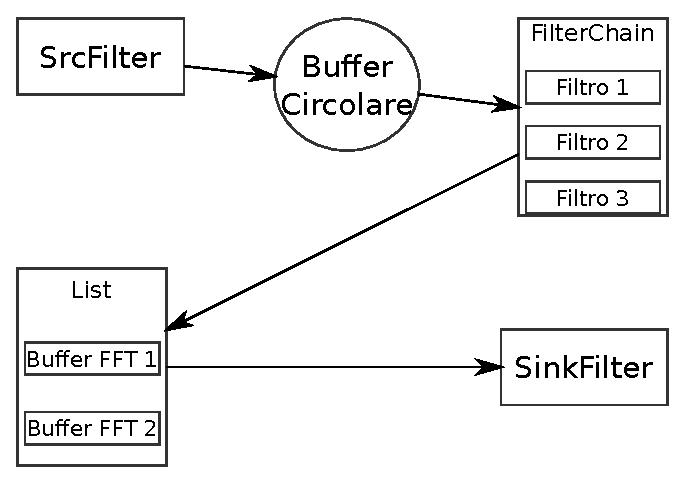
\includegraphics[width=1\linewidth]{algorithm}
	\end{center}
	\caption{Flusso dei dati all'interno del programma}
	\label{fig:algorithm}
\end{figure}

\subsection{SourceFilter}
\label{sourcefilter}
Una sorgente ha un unico metodo assolutamente necessario che serve a leggere i
dati. Una sottoclasse di \texttt{SourceFilter}, ad esempio, \`e il client UDP
(\texttt{udp\_sock}), che pu\`o essere usata da qualunque codice generico che
faccia riferimento unicamente all'interfaccia astratta. Se si creasse un'altra
sottoclasse di \texttt{SourceFilter} e la si sostituisse a \texttt{udp\_sock} si
otterrebbero i dati da un'altra fonte senza dover cambiare una riga di codice al
di fuori della inizializzazione.
\subsection{ProcessFilter}
Un \texttt{ProcessFilter} rappresenta una qualunque elaborazione intermedia del
segnale, sia essa una trasformata di Fourier o un filtro passa---basso o una
qualunque altra manipolazione. Siccome in questa fase si prende un segnale e lo
si manipola in qualche maniera, l'interfaccia richiede un metodo
\texttt{transform} che abbia in input i dati da elaborare e scriva su un vettore
di output specificato. I filtri sono per natura concatenabili, quindi per
gestire questa coda serve una classe \texttt{FilterChain} che si occupi di
passare l'elaborazione attraverso una coda di filtri precedentemente
selezionati.
\subsection{SinkFilter}
Le destinazioni hanno bisogno di un unico metodo di interfaccia: \texttt{write}.
In modo simile al \texttt{SourceFilter}, una qualunque implementazione della
classe astratta \texttt{SinkFilter} pu\`o essere intercambiata con un'altra
senza dover apportare modifiche al codice, permettendo di scegliere il
dispositivo di memorizzazione pi\`u adeguato agli scopi perseguiti.
\subsection{Contenitori di dati}
Sono state progettate alcune classi al fine di astrarre i dati e assicurarne la
corretta sincronizzazione.
\subsubsection{SrcType}
\texttt{SrcType} \`e una struttura con un costruttore, un destruttore ed un
operatore di assegnamento. Tra i membri di questa struttura c'\`e una mutex per
eseguire operazioni in mutua esclusione, ove necessario. Questa struttura \`e un
wrapper di un puntatore, ideale per essere usata all'interno di un circular
buffer.
\subsubsection{FFTBuf} La classe \texttt{FFTBuf} \`e un vettore su cui
vanno scritti i risultati di una o pi\`u trasformazioni di Fourier. Al momento
della costruzione, si indica la lunghezza del segnale da salvare e il numero di
integrazioni che si prevede di fare; a questa maniera \`e possibile assegnare
questo buffer a tanti thread quante dovranno essere le integrazioni da fare. La
classe offre strumenti anche per tener traccia di quante integrazioni sono già
state effettuate e sapere cos\`i se il buffer \`e pronto per essere scritto su
output.
\subsubsection{List}
La classe \texttt{List} \`e un semplice wrapper attorno ad una lista della
libreria standard. Questa classe assicura un comportamento corretto in ambienti
multithreading e aggiunge alcuni metodi per semplificare la coordinazione con
gli altri thread.

\subsection{Wrapper di librerie}
La classe \texttt{IPP} esiste solo per fornire un wrapper \CC alle librerie
\ac{ipp}, scritte in C. Tramite overloading \`e stato possibile utilizzare lo
stesso nome per funzioni che operano su tipi di dati differenti, lasciando al
compilatore il compito di invocare la funzione specifica pi\`u adeguata.

\section{Threading}
\begin{figure}[htb]
	\begin{center}
		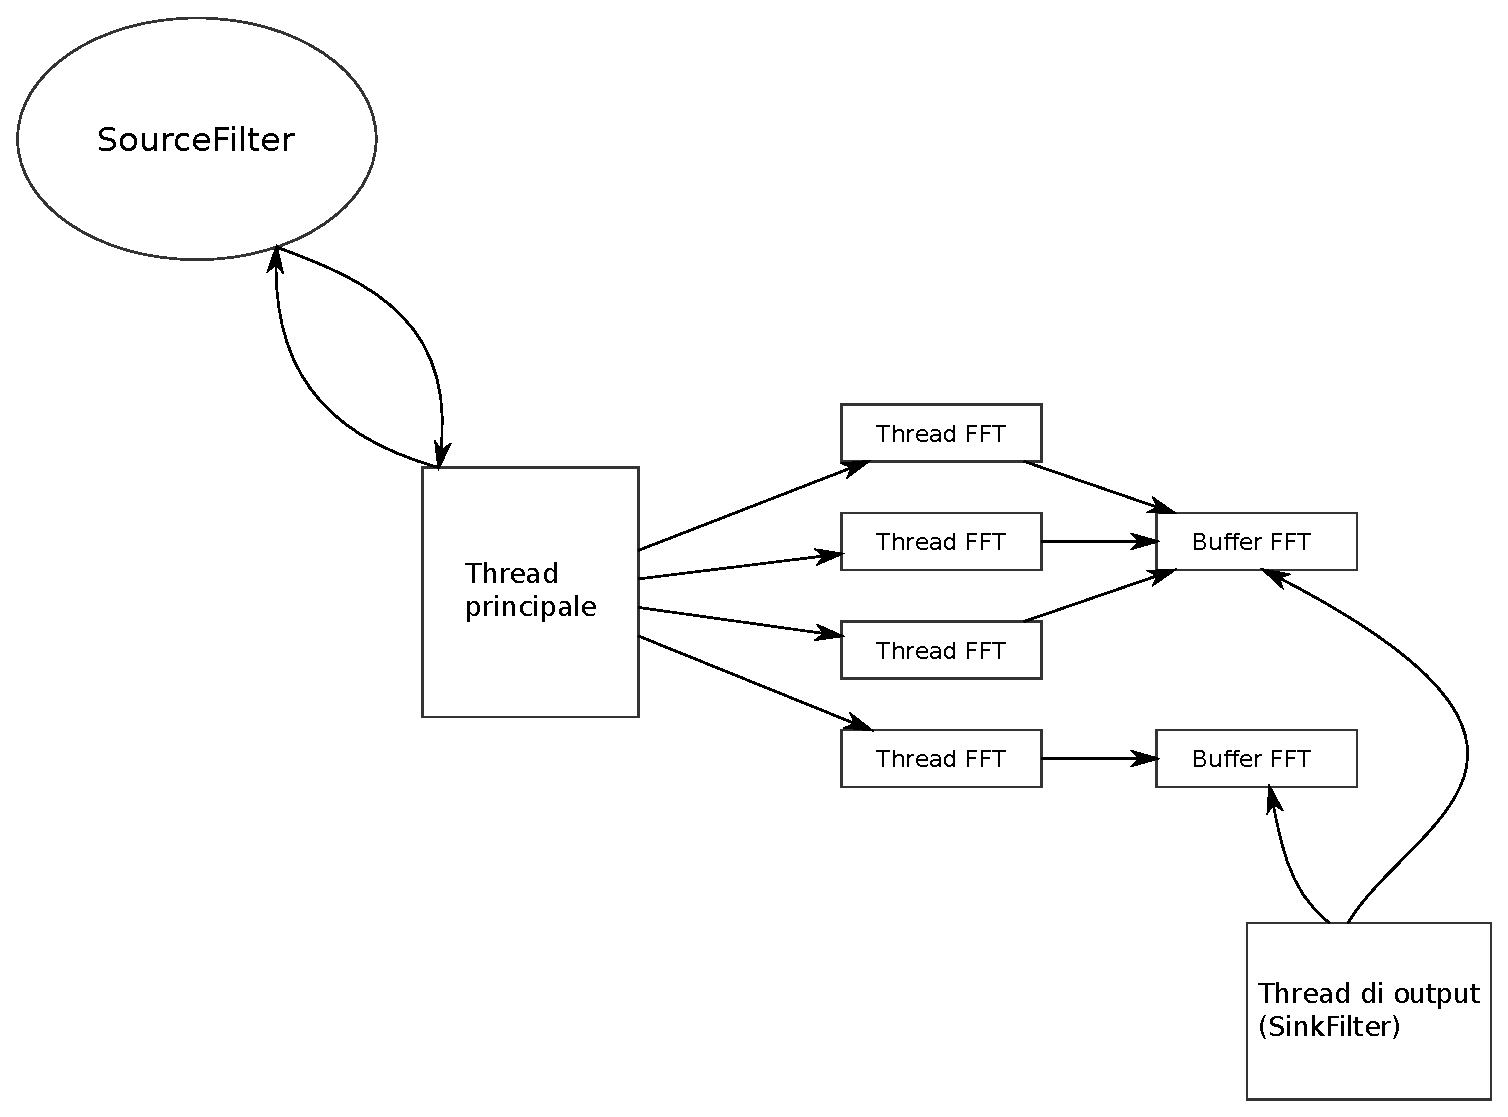
\includegraphics[width=1\linewidth]{threading}
	\end{center}
	\caption{Interazione dei diversi thread tra loro.}
	\label{fig:threading}
\end{figure}
Per incrementare le prestazioni soprattutto su elaboratori forniti di processore
multi-core o di pi\`u processori, il programma \`e stato progettato per
funzionare con differenti thread di esecuzione per le diverse parti. Questo
permette di sfruttare al massimo il processore senza dover attendere sui tempi
di lettura dei dati in ingresso (ad esempio, una rete locale) o sui tempi di
scrittura dei dati in uscita (ad esempio, un file locale). Inoltre \`e possibile
eseguire pi\`u di una trasformazione in parallelo, utile ad esempio nel caso in
cui si voglia sommare tra loro diversi segnali trasformati allo scopo di
attutire il rumore di fondo.

\subsection{Inizializzazione}
All'avvio dell'applicazione vengono lette le opzioni passate da linea di
comando, inizializzando le variabili con valori appropriati ed allocando alcuni
buffer. In seguito viene inizializzato un buffer circolare utilizzato per i
dati di input, una lista per i dati di output, un thread pool il cui compito
sar\`a calcolare le trasformazioni descritte dalla FilterChain ed un thread che
si occupa di scrivere l'output.

\subsection{Thread di output}
\label{threadout}
\begin{figure}[htb]
	\begin{center}
		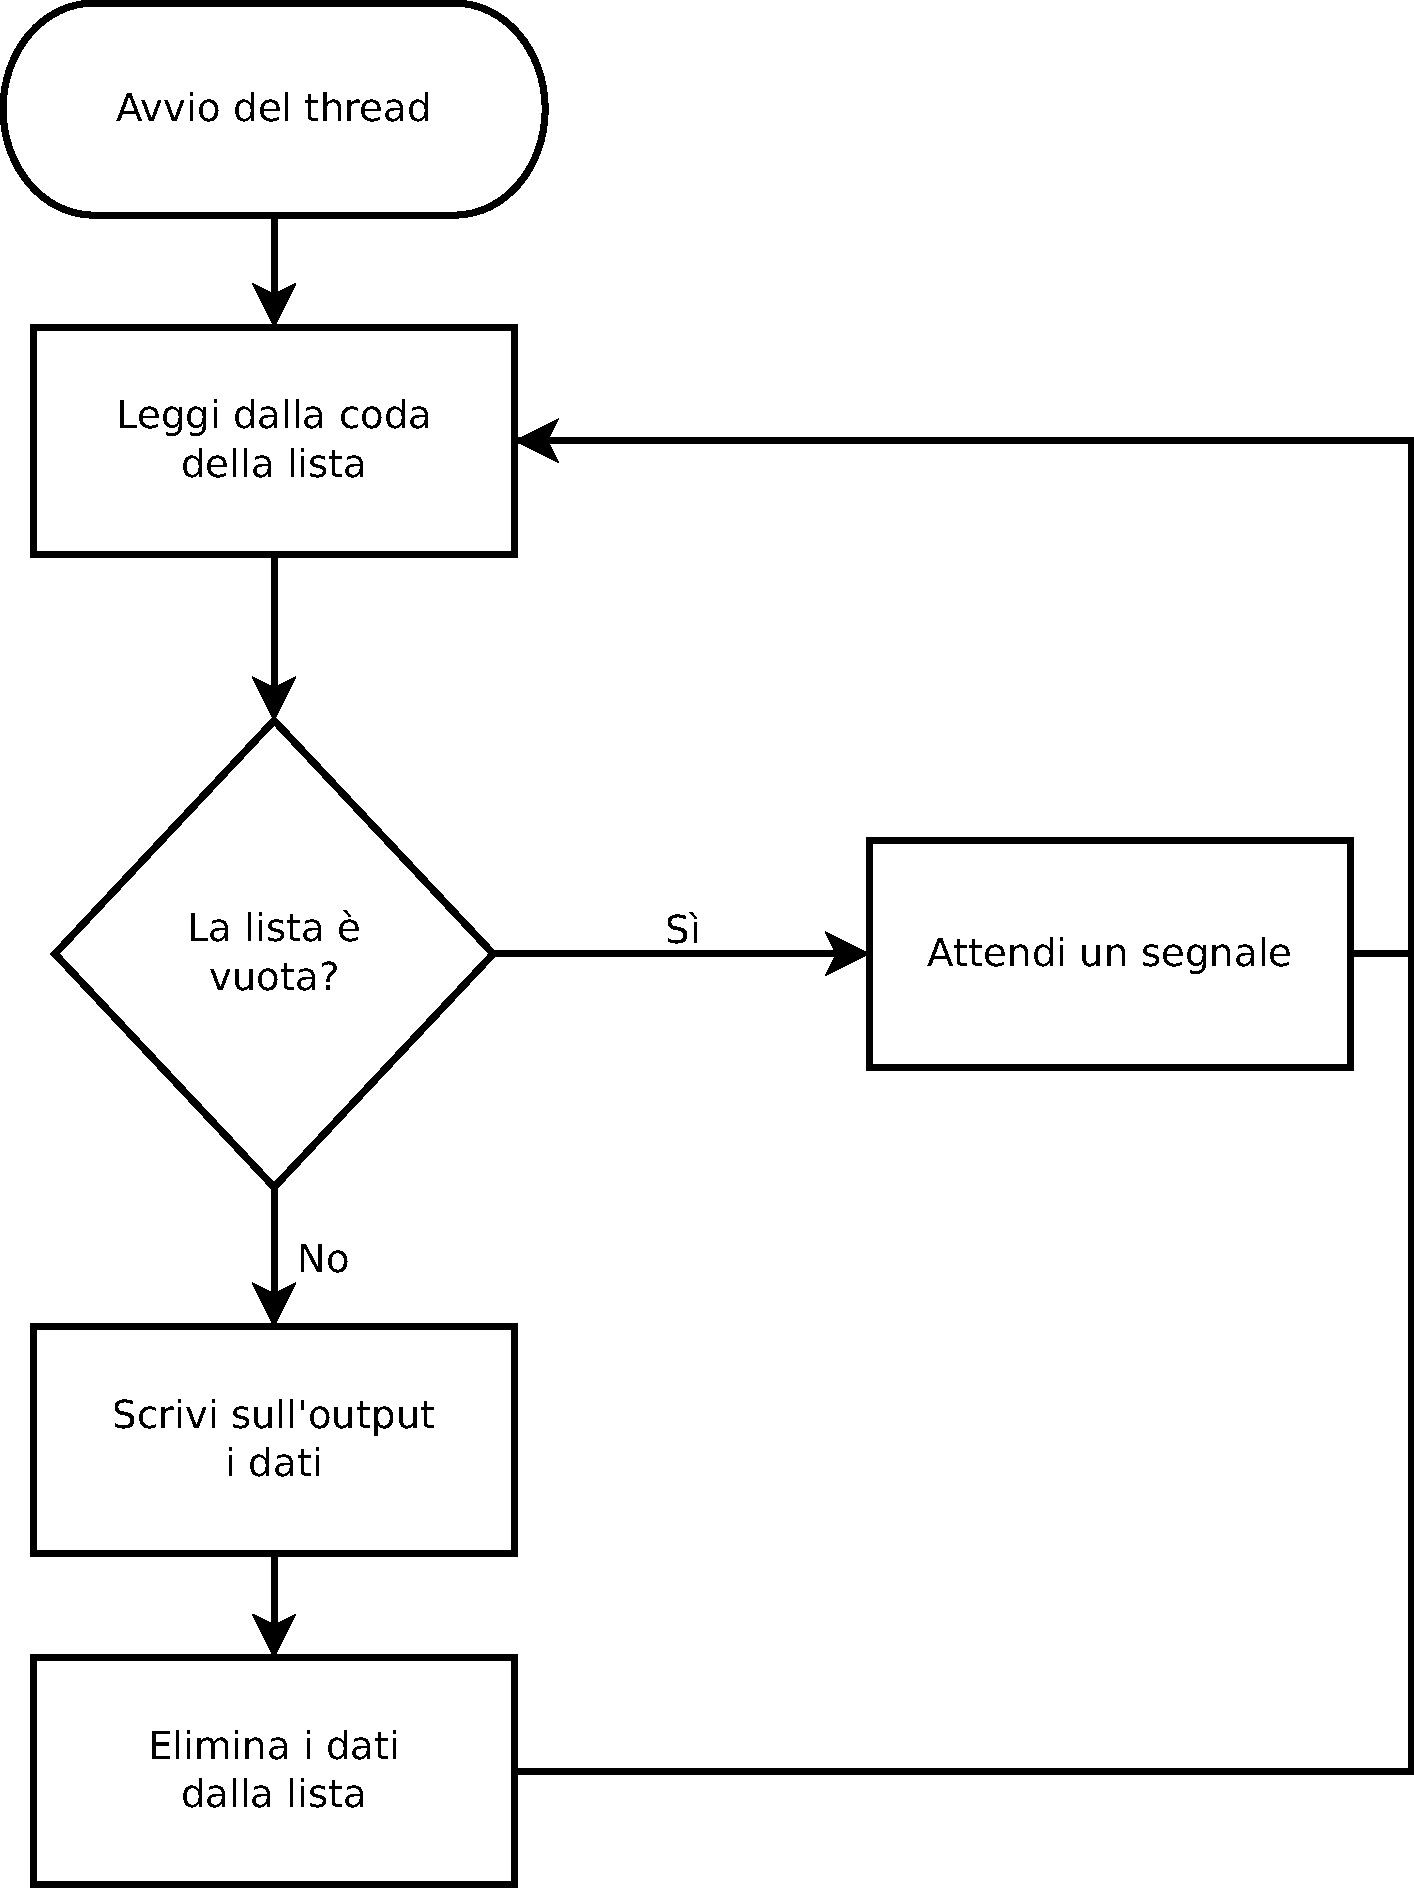
\includegraphics[width=1\linewidth]{output}
	\end{center}
	\caption{Algoritmo del thread di output}
	\label{fig:output}
\end{figure}
Il thread di output controlla i dati presenti in una lista, fornita durante
l'inizializzazione, dove verranno accodati i dati da scrivere in uscita. Quando
la lista \`e vuota, il thread si mette semplicemente in attesa, altrimenti
procede alla scrittura, rimuove dalla lista i dati scritti e ricomincia il
proprio ciclo da capo.

\subsection{Thread principale}
\label{main_thread}
Avviato il thread di output, il thread principale entra nel suo ciclo
principale, dove effettua tre operazioni che esploriamo nel dettaglio:
\emph{lettura dei dati}, \emph{selezione del buffer di output} e
\emph{assegnamento al thread pool}.
\subsubsection{Lettura dei dati}
La prima operazione effettuata all'interno del ciclo principale \`e verificare
che ci sia dello spazio disponibile nel buffer circolare. Se il buffer \`e
pieno --- cio\`e se tutti i dati nel buffer devono ancora essere elaborati ---
il thread si mette in attesa che il carico di lavoro venga smaltito. Quando
c'\`e dello spazio disponibile nel buffer circolare, si leggono i dati
dal SourceFilter e si accodano. Si procede poi alla selezione del buffer di
output.
\subsubsection{Selezione del buffer di output}
Una volta ottenuti i dati da elaborare, si verifica se esistono buffer accodati
nella lista di output. Se non ce ne sono, si crea un nuovo buffer, lo si accoda
alla lista e lo si seleziona come buffer di output; se, invece, la lista
contiene dei buffer si seleziona il buffer di testa e si verifica se \`e
utilizzabile o meno: siccome allo scopo di attutire il rumore di fondo in un
segnale spesso di fanno le somme di diversi segnali trasformati, esiste un
parametro che determina quante di queste somme si vogliono effettuare. Per ogni
buffer si tiene traccia del numero di thread a cui \`e stato assegnato e se
questo numero \`e minore rispetto al numero di somme desiderate, il buffer \`e
selezionabile, altrimenti se ne crea uno nuovo e lo si accoda in lista.
\subsubsection{Assegnazione al thread pool}
Dopo aver letto i dati del segnale da trasformare ed aver individuato il buffer
di output su cui scrivere i dati elaborati, si può assegnare il lavoro al thread
pool. Per farlo, \`e sufficiente indicare i puntatori ai due buffer ed un
puntatore alla funzione che deve occuparsi di elaborare i dati. Il thread pool
si occuper\`a automaticamente di assegnare il lavoro al primo thread libero
presente nel suo pool.

\chapter{Sviluppo del progetto}
\label{sw_devel}

Durante lo sviluppo del progetto si ha fatto uso di librerie e strumenti
software per semplificare il pi\`u possibile il lavoro da svolgere ed ottenere
il massimo delle prestazioni possibili. 

\section{Librerie}
L'utilizzo delle giuste librerie permette di sviluppare pi\`u velocemente i
propri progetti, ottenere prestazioni spesso migliori rispetto ad una soluzione
sviluppata in proprio e sicuramente avere pi\`u certezze riguardo al corretto
funzionamento delle parti attenenti alla libreria.

\subsection{Boost}
Le librerie Boost\footnote{\url{http://www.boost.org/}} sono molto usate nella
programmazione in \CC perch\'e implementano moltissime funzioni di comune
utilizzo fornendo una interfaccia molto semplice. L'ottima qualit\`a di queste
librerie \`e confermato dal fatto che spesso alcune sue componenti vengono
integrate nello standard \CC. Queste librerie sono basate sulla versione ANSI
del \CC, rendendole compatibili con qualunque compilatore che implementi gli
standard ANSI.In questo progetto vengono utilizzate principalmente per
semplificare la lettura di argomenti da linea di comando, la lettura/scrittura
di files, le comunicazioni di rete e il multithreading.

\subsection{\ac{ipp}}
Le Integrated Performance
Primitives\footnote{\url{http://software.intel.com/en-us/intel-ipp/}} sono delle
librerie che implementano un insieme molto completo di funzioni e algoritmi
relativi al processamento di segnali e crittografia. In particolare implementano
funzioni utili al processamento di segnali audio (filtri, codifiche audio,
compressione dei dati, ecc.), funzioni per il processamento di immagini
(trasformazioni, codifica video, ecc.), funzioni per calcoli su matrice e
funzioni crittografiche (crittografia simmetrica, asimmetrica, funzioni hash,
ecc.).  Il vantaggio delle IPP \`e che offrono un ampio spettro di funzioni che
coprono praticamente tutte le necessit\`a nel processamento dei segnali, oltre
ad essere ottimizzate per processori Intel. Inoltre sono state scritte in modo
da essere naturalmente utilizzabili in ambienti multithreaded, sfruttando tutte
le potenzialit\`a di processori multicore o processori multipli. Tutti questi
fattori hanno concorso nell'adozione di questa libreria al posto di altre
librerie concorrenti. Questa libreria \`e l'unico componente non Open Source
utilizzato nell'intero progetto, anche se il suo utilizzo \`e gratuito per usi
accademici. Le librerie alternative potrebbero essere comparate per verificare
l'effettiva qualit\`a a livello di prestazioni\footnote{cfr. paragrafo
\ref{altlib}}.

\subsubsection{Multithreading e prestazioni nelle \ac{ipp}}
Le \ac{ipp} sono state sviluppate con l'intenzione di sfruttare a pieno le
istruzioni \ac{SIMD} e \ac{SSE} presenti nei moderni processori. Queste
istruzioni permettono di effettuare operazioni su vettori in parallelo,
guadagnando grandi vantaggi prestazionali in alcuni tipi di operazioni, tra cui
anche i calcoli necessari per l'elaborazione di segnali. Siccome diversi
processori supportano diversi tipi di istruzioni, possono esistere diverse
implementazioni di alcune funzione in base al tipo di istruzioni supportate. Per
selezionare automaticamente la funzione corretta, le \ac{ipp} dispongono di un
dispatcher che, durante l'inizializzazione a run-time, individuano le capacit\`a
del processore e quindi la categoria di libreria da utilizzare. Questo permette
di usare trasparentemente le funzioni di libreria sfruttando sempre
l'implementazione pi\`u efficiente per il processore utilizzato.

Alcune funzioni di base della libreria sfruttano il threading per migliorare le
proprie prestazioni, in particolare sfruttando le librerie OpenMP sviluppate da
Intel. Quando si utilizza la versione multi-threaded della libreria, i thread
vengono automaticamente inizializzati al numero di processori e core presenti: a
questo modo la libreria avvier\`a al massimo tanti thread quante sono le unit\`a
di calcolo presenti nel sistema, evitando di sovracaricare il sistema e
ottenendo cos\`i la migliore prestazione possibile dal sistema in uso. Sono
presenti anche due funzioni, \texttt{ippSetNumThreads()} e
\texttt{ippGetNumThreads()}, che permettono di manipolare il numero di threads
utilizzati dalla libreria. Il numero di thread non sar\`a mai maggiore rispetto
al numero di unit\`a di calcolo del sistema, anche se impostati manualmente ad
un valore maggiore.

Tutte le funzioni IPP sono thread safe, cio\`e possono essere usate da diversi
thread di esecuzione contemporaneamente senza che questo implichi un qualunque
malfunzionamento.\footnote{Per approfondimenti, cfr.
\url{http://software.intel.com/en-us/articles/threading-and-intel-integrated-performance-primitives/}}


\section{Codice pre-esistente}
Parte del codice del progetto \`e stato prelevato dal software sviluppato in
fase di tirocinio, sempre presso l'Istituto di Radioastronomia di Medicina.
Questo codice ha permesso di ridurre notevolmente il tempo dedicato allo
sviluppo del calcolo della \ac{FFT} lasciando maggior tempo per una corretta
implementazione delle altre parti. Questo codice \`e stato adattato per
funzionare in un contesto multithreaded e per accettare input da diverse fonti.

\section{Gestione del threading}
Quando si introduce il threading in una applicazione, ci sono delle situazioni
che vanno prese in considerazione: avere diversi thread pu\`o portare problemi
normalmente assenti e non facilmente identificabili. Inoltre alcuni problemi
legati al threading possono essere difficili da riprodurre perch\'e  dipendono
dalla schedulazione dei thread da parte del sistema operativo, quindi 
\subsection{Mutua esclusione}
\subsection{Wait/notify}
\subsection{Debugging}

\chapter{Risultati e considerazioni}
\label{tests}
Una volta terminato lo sviluppo dell'applicazione e verificato che non ci siano
problemi durante l'esecuzione, sono stati eseguiti diversi test per verificare
correttezza e prestazione dell'applicazione.

\section{Correttezza dell'applicazione}
Per verificare la correttezza dell'applicazione si visualizza un segnale
trasformato dal programma; questo segnale \`e noto o comunque si conosce la
forma approssimativa che si dovrebbe ottenere, come accennato nel paragrafo
\ref{pyvis}. In figura \ref{fig:correctness} si vede la visualizzazione di un
segnale con larghezza di banda di 5 Mhz ed elaborato a 4096 canali di frequenza.
Come si vede dalla figura, tra i canali 1000 e 3100 circa c'\`e una grande curva
con piccoli picchi sopra di essa. La curva, o \emph{panettone}, rappresenta una
elaborazione del segnale: prima di arrivare allo spettrometro, il segnale \`e
pre-processato con alcuni filtri che gli danno l'aspetto in figura. I dati
rilevanti sono quelli presenti sulla zona piatta in cima al panettone, mentre i
picchi presenti sopra il panettone rappresentano verosimilmente delle
interferenze.

Va notato che uno strumento di misura introduce un qualche tipo di
``distorsione'' detta \emph{bandshape}, o banda caratteristica del ricevitore.
Questo implica che nell'interpretazione di un segnale va considerata questa
bandshape per evitare di trarre conclusioni erronee sulla natura del segnale:
normalmente \`e possibile ``correggere'' il segnale registrato in modo da
ottenere la forma reale del segnale stesso.
\begin{figure}[htb]
	\begin{center}
		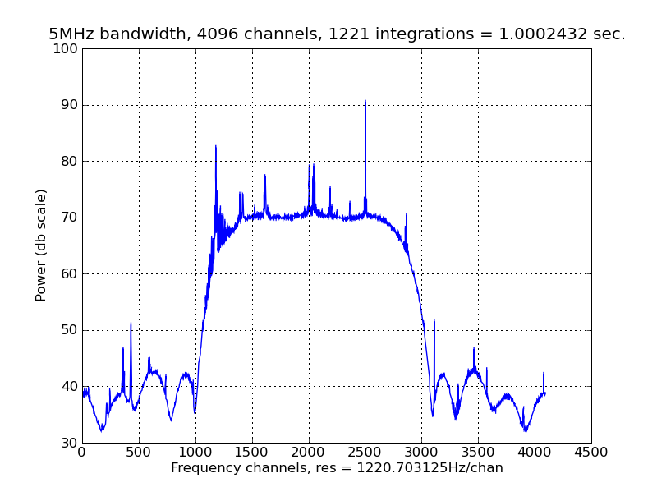
\includegraphics[width=1\linewidth]{5_4096_1221}
	\end{center}
	\caption{Visualizzazione di un segnale elaborato con il programma}
	\label{fig:correctness}
\end{figure}

Da questa immagine si capisce quindi che il programma elabora correttamente i
dati e produce una trasformazione corretta dei segnali.

\subsection{Riduzione del rumore}
Verifichiamo anche il corretto funzionamento del metodo delle somme dello stesso
segnale per attutire il rumore: nella figura \ref{fig:low_int} si vede un
segnale con 5 Mhz di banda ed elaborato a 512 canali, senza effettuare alcuna
somma di altre elaborazioni. Si pu\`o osservare con il grafico risultante sia
estremamente frastagliato e a malapena si riesce ad intuire la forma del
segnale, mentre le eventuali interferenze non sono nemmeno distringuibili dal
rumore di fondo.
\begin{figure}[htb]
	\begin{center}
		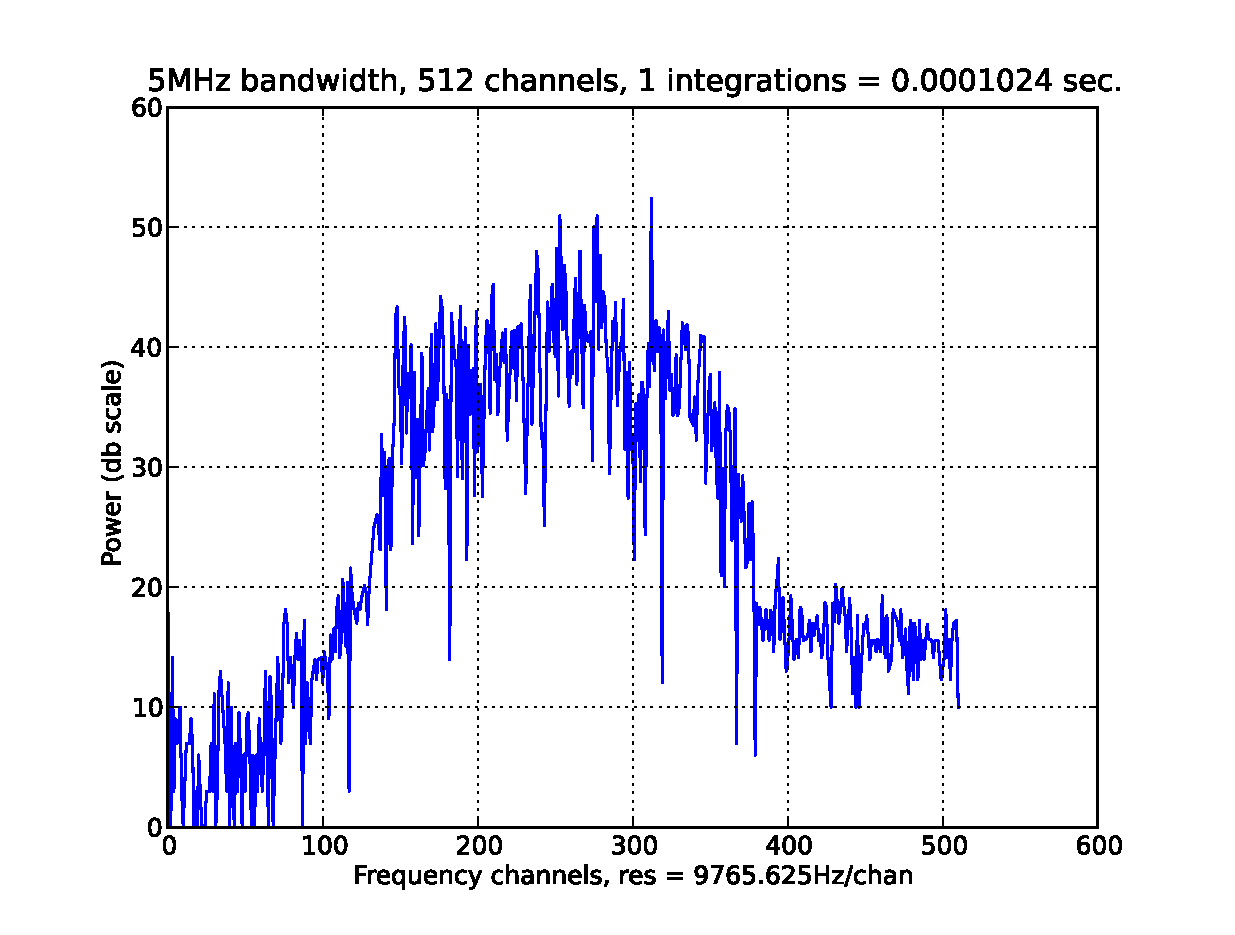
\includegraphics[width=1\linewidth]{5_512_1}
	\end{center}
	\caption{Segnale senza nessuna integrazione}
	\label{fig:low_int}
\end{figure}

Confrontiamo questa immagine con la figura \ref{fig:high_int} dove vengono
effettuate 97656 elaborazioni successive di un segnale nel tempo e poi sommate
tra di loro: in questa seconda immagine \`e perfettamente delineata la forma del
segnale cos\`i come sono perfettamente visibili le interferenze presenti.  Si
intuisce anche come le due immagini rappresentino la stessa cosa, anche se la
prima \`e un po' ``sfuocata'', non sufficientemente dettagliata, mentre la
seconda \`e molto pi\`u netta. Questo avviene perch\'e integrando un segnale
periodico migliora il rapporto segnale/rumore (SNR).
\begin{figure}[htb]
	\begin{center}
		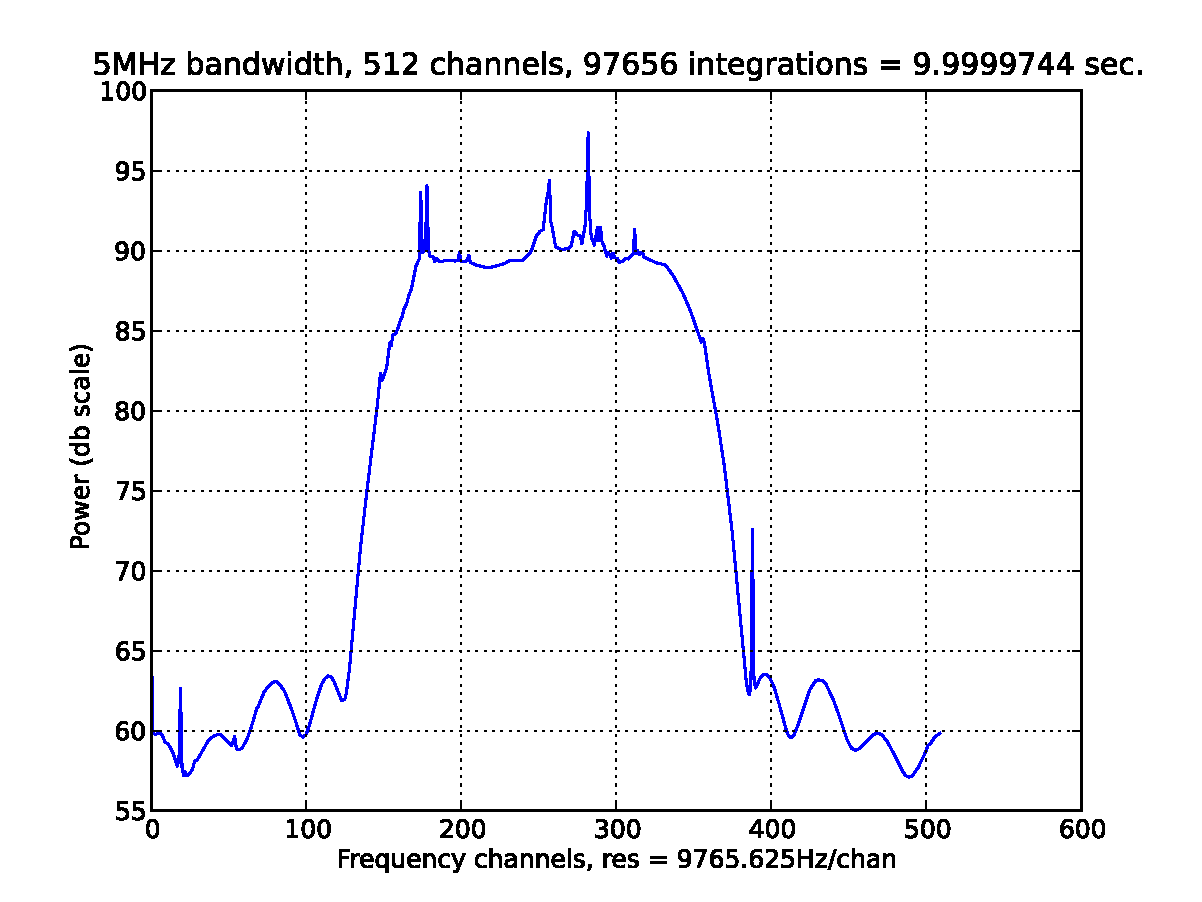
\includegraphics[width=1\linewidth]{5_512_97656}
	\end{center}
	\caption{Segnale con un elevato numero di integrazioni}
	\label{fig:high_int}
\end{figure}

Tuttavia va considerato anche che aumentando il numero di somme, aumenta anche
il tempo di elaborazione necessario: nel primo caso per calcolare i dati
rappresentati nell'immagine \`e stato richiesto un tempo di $0,0001$ secondi,
mentre nel secondo caso sono stati impiegati $10,9$ secondi.  Chiaramente va
ricercato un compromesso tra riduzione del rumore e tempo di calcolo,
compromesso che varia a seconda del tipo di analisi che si desidera fare: per
alcuni tipi di osservazioni va bene anche un segnale non molto ben definito,
purch\'e sia calcolato molto in fretta; per altri tipi di osservazioni, il
segnale deve essere definito molto precisamente, al costo di un maggiore tempo
di calcolo.

\subsection{Variazione del numero di canali}
Il numero di canali usati nel calcolo della \ac{FFT} influiscono sulla
risoluzione di ognuno di questi canali: se i canali sono pochi, ogni canale
rappresenta una banda di frequenza piuttosto ampia, mentre con molti canali la
banda di frequenza si restringe. Aumentare il numero di canali permette di
analizzare un segnale pi\`u nel dettaglio, osservando anche variazioni tra
frequenze molto vicine tra loro. Al contrario, con pochi canali l'energia del
segnale viene distribuita in porzioni di banda vicine tra loro. Per verificare
questo fenomeno, si confrontino la figura \ref{fig:low_chans} con la figura
\ref{fig:high_chans}: nella seconda figura tutta la zona colorata di blu \`e
composta da oscillazioni vicinissime tra loro, presenti anche nella prima
figura, ma abbastanza distanziate da essere ben visibili. Nella prima figura,
ogni canale ha una risoluzione di $19531,25 Hz/canale$, mentre nella seconda
ogni canale ha una risoluzione di $1,192 Hz/canale$.
\begin{figure}[htb]
	\begin{center}
		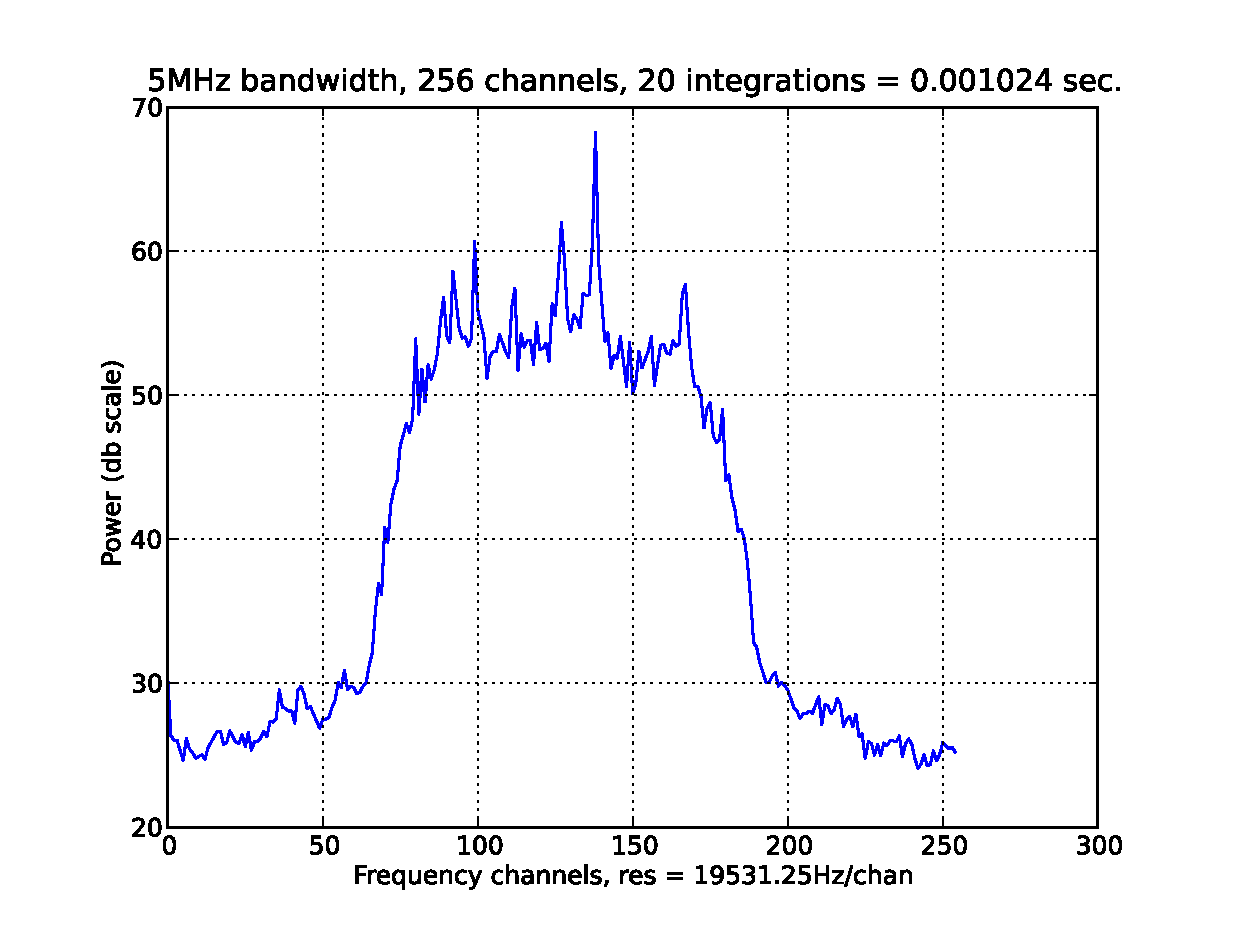
\includegraphics[width=1\linewidth]{5_256_20}
	\end{center}
	\caption{Segnale analizzato con pochi canali}
	\label{fig:low_chans}
\end{figure}

\begin{figure}[htb]
	\begin{center}
		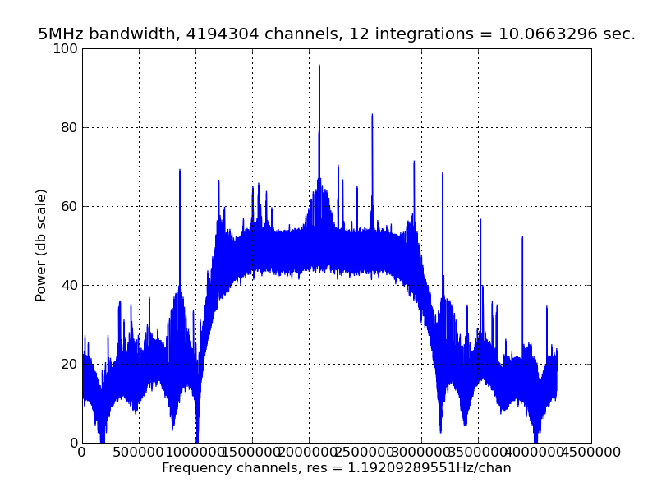
\includegraphics[width=1\linewidth]{5_4194304_12}
	\end{center}
	\caption{Segnale analizzato con molti canali}
	\label{fig:high_chans}
\end{figure}

Come per la riduzione del rumore di fondo, aumentando il numero di canali
aumenta il tempo di calcolo; allo stesso modo il compromesso tra numero di
canali e tempo di calcolo dipende dal tipo di analisi che si intende effettuare.

\section{Verifica delle prestazioni}
\subsection{Caratteristiche dell'elaboratore}
Nel verificare le prestazioni del programma, \`e importante tenere in
considerazione il tipo di elaboratore su cui vengono effettuati questi test. Il
server collegato ai dati provenienti dall'antenna ha un processore Intel (???),
4(???) Gb di memoria RAM e come sistema operativo Ubuntu Linux (???). \`E
collegato ad una rete a 10 Gbit/s con i Jumbo Frames\footnote{???} attivati.
Tutti i segnali su cui si sono effettuati i test contenevano valori di 16 bit
per ogni punto, con banda del segnale di 5 Mhz.
\subsection{Tests eseguiti}
\ctable[
    cap=Alcuni tempi di calcolo,
    caption=Esempio di alcuni tempi di calcolo,
    label=tab:tests
]{llllll}{
\tnote[a]{Tempo espresso in secondi}
\tnote[b]{Dimensione dei files in bytes}
\tnote[c]{Si intende il tempo impiegato per effettuare tutte le \ac{FFT} e le somme dei risultati.}
}{
                \FL
Can. & Integr. & Tempo totale\tmark[a] & Dim. output\tmark[b] & Segnali output & Tempo trasf.\tmark[a]\tmark[c] \ML
256 & 1 & 4.831 & 96423936 & 94164 & 5.13041e-05\NN
256 & 20 & 5.984 & 5974016 & 5834 & 0.00102571\NN
256 & 195 & 3.952 & 403456 & 394 & 0.0100305\NN
256 & 195313 & 24.182 & 2048 & 2 & 12.091\NN
512 & 1 & 5.087 & 101545984 & 49583 & 0.000102596\NN
512 & 98 & 9.040 & 1841152 & 899 & 0.0100556\NN
65536 & 1 & 5.115 & 101974016 & 389 & 0.0131491\NN
65536 & 76 & 6.267 & 1572864 & 6 & 1.0445\NN
524288 & 1 & 3.962 & 77594624 & 37 & 0.107081\NN
524288 & 95 & 38.645 & 6291456 & 3 & 12.8817\NN
4194304 & 1 & 6.242 & 100663296 & 6 & 1.04033\NN
4194304 & 12 & 38.022 & 50331648 & 3 & 12.674\LL
}

Una volta determinato che il programma funziona, \`e stabile e produce dei
risultati corretti, si pu\`o verificare il livello di prestazioni. Per questo
sono stati fatti dei test dove si aumentava man mano il numero di canali e il
numero di integrazioni. L'aumento del numero di integrazioni \`e stato studiato
in modo che l'ordine di grandezza del tempo di calcolo previsto aumentasse ad
ogni test: se si osserva le prime righe della tabella \ref{tab:tests_256} si nota
che all'aumentare del numero di integrazioni il tempo si moltiplica all'incirca
per 10.\footnote{Notare che nella prima riga si impiega 20 volte meno tempo
    rispetto alla seconda. Questo perch\'e le integrazioni avrebbero dovuto
    essere 2 per ottenere un tempo 10 volte inferiore.}
Per valutare il numero di integrazioni necessarie, la formula utilizzata \`e
$integrations = \frac{bandwidth}{channels} * time$. Considerando che tutti i
segnali utilizzati hanno 5 Mhz di banda, \`e facile ricavare il numero di
integrazioni richieste. I tempi testati oscillano tra $10^{-3}$ e $10$.
I canali aumentano raddoppiando, per motivi visti nel paragrafo
\ref{analisi_sintesi}, e ogni volta che si incrementa il numero di canali,
conseguentemente incrementa il tempo di calcolo.

L'obiettivo di questi test \`e di verificare un eventuale limite superiore del
programma nel calcolare le trasformate. Avendo predeterminato i tempi di calcolo
desiderati, \`e facile verificare la tenuta dell'algoritmo: si osservino le
tabelle nell'appendice \ref{test_tables}, si noter\`a che tutti i tempi
rientrano nelle previsioni.

Si \`e arrivati a testare al massimo $2^{22} = 4194304$ canali perch/'e essendo il
segnale a 5 Mhz di banda, non avrebbe senso analizzarlo ad una risoluzione
minore di $1 \frac{Hz}{canale}$. Tuttavia per verificare in quali condizioni il
programma smette di funzionare, si sono effettuati dei test con un numero di
canali ancora maggiore, arrivando sino a $2^{27} = 134217728$ canali: attorno ai
valori $2^{26}$--$2^{27}$ il programma non riesce ad allocare tutta la memoria
necessaria all'elaborazione. Inoltre elaborando a $2^{25}$ canali si inizia a
perdere qualche pacchetto UDP dalla rete, segno che il processore non riesce ad
elaborare il segnale con sufficiente rapidit\`a. Con questi limiti, il programma
\`e in grado di elaborare segnali fino a 20 Mhz di banda e, con un hardware
pi\`u potente, potrebbe essere possibile elaborare segnali a banda ancora pi\`u
larga, ben oltre le reali necessit\`a.

\chapter{Conclusioni e sviluppi futuri}
\label{conclusions}
\section{Conclusioni}
Lo scopo principale dello sviluppo di questo programma \`e capire che tipo di
prestazioni ci si pu\`o aspettare da una soluzione software all'elaborazione di
segnali radioastronomici. Basandosi sui risultati dei test, si vede che il
programma \`e in grado di elaborare correttamente delle quantit\`a importanti di
dati; se confrontate con le prestazioni di una macchina DSP\footnote{DSP
    significa, in questo caso, Digital Signal Processor. Con questo nome si
    indicano degli elaboratori specializzati che effettuano solamente le
    trasformate per cui sono costruiti.} sicuramente saranno inferiori, ma se si
aggiunge al confronto anche i fattori del costo dell'attrezzatura e la
flessibilit\`a della soluzione alle esigenze si capisce come le prestazioni di
questo software siano importanti: il software lavora su un normale elaboratore
il cui prezzo, nel caso di macchine comunque high-end e piuttosto potenti, si
aggira attorno ai 6000 euro. L'hardware specializzato per il DSP ha costi molto
pi\`u elevati, nell'ordine dei 10000 euro, anche se spesso i consumi sono
minori. Inoltre, modificare un programma scritto in \CC\, \`e un'operazione
relativamente semplice e che molte persone sono in grado di fare, mentre per
modificare l'algoritmo in una macchina DSP bisogna modificare l'hardware,
operazione per nulla semplice, n\'e rapida, quindi anche pi\`u costosa. Avere
una soluzione un po' meno performante, ma comunque di buon livello a costi
contenuti \`e importante sia in quei campi di ricerca dove le prestazioni non
sono un aspetto fondamentale del lavoro, sia per progetti a budget molto
ristretto, dove avere degli strumenti a basso costo \`e fondamentale.
Un altro aspetto importante \`e il fatto che un elaboratore generico pu\`o
essere riutilizzato per altri scopi, ad esempio alla fine del progetto o nei
tempi ``morti'' in cui non serve fare elaborazioni sui segnali, mentre hardware
specifico per il DSP \`e difficile da riutilizzare in altri ambiti.

\section{Sviluppi futuri}
Gli ottimi risultati conseguiti aprono la strada a diversi sviluppi possibili:
si può adattare il programma ad altri scopi, provare implementazioni diverse,
cercare di migliorarne ancora le prestazioni e tanto altro ancora.
\subsection{Estensione del programma}

\subsubsection{Implementazione di altre trasformazioni}
Il modo pi\`u semplice per estendere le funzionalit\`a del programma \`e
scrivere qualche trasformazione o filtro aggiuntivo da accodare nella
\texttt{FilterChain}. Essendo gi\`a pronte le interfacce, ed esistendo gi\`a una
sua implementazione, la parte di lavoro necessaria riguarda solamente la
scrittura delle funzioni di trasformazione, senza dover sviluppare un modo per
gestire il flusso dei dati.

\subsubsection{Selezione dinamica del tipo di dato}
\label{dyn_dtype}
Nell'implementazione attuale, la selezione del tipo di dati in ingresso ed in
uscira \`e basato su delle costanti all'interno del codice. Per modificare
queste costanti bisogna modificare il programma e ricompilarlo, operazione che,
per quanto semplice, potrebbe essere rimossa completamente permettendo di
selezionare il tipo di dato ad esempio da linea di comando.

\subsubsection{Controllo interattivo dei parametri}
Un altro possibile sviluppo del programma \`e la possibilit\`a di controllare in
modo interattivo i parametri del programma ed avviare/fermare il processo
tramite una console accessibile tramite rete. Il funzionamento \`e piuttosto
semplice: connettendosi tramite rete alla console, si possono impartire vari
comandi per modificare il tipo di trasformazioni effettuate ed i loro parametri,
la fonte di acquisizione e la destinazione dei dati. Si può anche avviare e
fermare il ciclo principale di elaborazione e leggere delle statistiche sul suo
funzionamento.

\subsubsection{Output di rete}
Attualmente l'unica implementazione del \texttt{SinkFilter} \`e una classe che
scrive l'output su file. Molto utile potrebbe essere la scrittura su una
interfaccia di rete, cos\`i che i dati possano essere letti da un computer
remoto. Questo permetterebbe anche di visualizzare i dati in tempo reale
spostando sul client il programma di visualizzazione.

\subsubsection{Acquisizione dati \ac{seti}}
\label{seti}
L'acquisizione di dati per il progetto \ac{seti} non avviene tramite rete, ma
utilizza uno speciale hardware dedicato. Leggere i dati da questo hardware
richiede un certo lavoro via software che potrebbe essere integrato all'interno
dell'interfaccia \texttt{SourceFilter}, cos\`i che il programma possa essere
utilizzato per elaborare i dati per il progetto \ac{seti}.

\subsection{Librerie alternative}
\label{altlib}

Esistono diverse liberie alternative alle \ac{ipp} che svolgono le stesse
operazioni. Per avere parametri di confronto, sarebbe interessante utilizzarle
nello stesso tipo di programma per verificare se effettivamente le
ottimizzazioni presenti nelle \ac{ipp} offrono grandi vantaggi rispetto ad
implementazioni alternative.

\subsubsection{FFTW: The Fastest Fourier Transform in the West}
La libreria FFTW \`e un progetto Open Source che sostiene di avere la pi\`u
rapida implementazione della \ac{FFT}.

\subsubsection{Framewave}
La libreria Open Source Framewave \`e stata sviluppata da AMD per fare
concorrenza alle \ac{ipp}. L'interfaccia di Framewave \`e molto simile a quella
delle \ac{ipp}, rendendo quindi pi\`u semplice l'adattamento del programma
all'utilizzo di questa libreria.

\subsubsection{\ac{FFT} sulla GPU}
Esistono diverse librerie che invece di sfruttare il processore per calcolare la
\ac{FFT}, utilizzano la GPU della scheda grafica. Alcuni
benchmark\footnote{\url{http://www.cv.nrao.edu/~pdemores/gpu/}} mostrano un
miglioramento interessante delle prestazioni rispetto a librerie per CPU,
soprattutto con l'aumentare il numero di canali. Esistono diverse librerie che
permettono di sfruttare la GPU, tra cui
CUDA\footnote{\url{http://www.nvidia.com/object/cuda_home_new.html}} e
GPUFFTW\footnote{\url{http://gamma.cs.unc.edu/GPUFFTW/}}. Se queste librerie si
dovessero mostrare realmente efficaci, i requisiti hardware si limiterebbero
fondamentalmente alla scheda grafica, permettendo di ridurre ulteriormente il
costo di una soluzione software.

\subsection{Compilatori}
Un altro aspetto da esplorare sono i compilatori: nel progetto \`e stato
utilizzato il compilatore g++, parte della suite di compilatori GNU gcc, con le
sue opzioni standard. Siccome dalla qualit\`a del compilatore e dalle opzioni
utilizzate dipende anche la qualit\`a del codice macchina generato e quindi la
sua rapidit\`a, un miglioramento di prestazioni potrebbe essere possibile
esplorando diverse opzioni.

\subsubsection{GCC/g++}
Il compilatore GNU gcc, nella sua versione per il \CC\, g++, \`e il pi\`u
diffuso in ambiente *NIX. Supporta numerose architetture e per ogni architettura
ha delle specifiche opzioni per ottimizzare il codice prodotto. Siccome nel
progetto \`e stato utilizzato senza particolari opzioni, sarebbe interessante
verificare se \`e possibile spremere prestazioni migliori con l'utilizzo delle
funzionalit\`a avanzate di g++.

\subsubsection{ICC}
Il compilatore ICC \`e stato sviluppato da Intel ed \`e il compilatore con cui
sono state compilate le liberie \ac{ipp} stesse. Essendo stato sviluppato
dall'azienda produttrice di processori, potrebbe essere in grado di sfruttare
molto meglio l'architettura dei processori Intel rispetto ad altri compilatori.

\subsubsection{Clang e LLVM}
Clang e LLVM formano insieme un compilatore e la sua interfaccia; sono un
progetto relativamente giovane e sono stati sviluppati da Apple con una licenza
di tipo BSD. Questo nuovo compilatore sembra produrre codice molto più rapido
rispetto gli altri compilatori e sta guadagnando un seguito molto importante
nella comunit\`a FreeBSD e non solo.

\subsection{Altri sviluppi}
La natura modulare del programma lo prestano ad un'infinit\`a di manipolazioni
ed utilizzi nuovi. Con i dovuti arrangiamenti potrebbe addirittura essere
utilizzato per scopi completamente differenti, come ad esempio la codifica di
file audio o l'elaborazione di immagini. A seconda delle necessit\`a si possono
apportare piccoli miglioramenti e l'architettura pensata cerca di essere il
pi\`u possibile flessibile verso esigenze diverse. Come per ogni progetto
software, le vere potenzialit\`a ed i veri limiti diventeranno evidenti
solamente nel tempo e tentando di utilizzare il programma negli ambiti pi\`u
differenti.


\bibliographystyle{alpha}
\bibliography{thesis}
\end{document}
